\documentclass{article}

\usepackage{cite}
\usepackage{amsmath,amssymb,amsfonts}
\usepackage{algorithmic}
\usepackage{graphicx}
\usepackage{textcomp}
\usepackage{xcolor}
\usepackage{relsize}
\usepackage[left=3.5cm,right=3.5cm]{geometry}
\usepackage{hyperref}
\usepackage{algorithm}
\usepackage{algorithmic}
\usepackage{authblk}
\usepackage[italian]{babel}
\usepackage{subcaption}
\usepackage{multirow}
\usepackage{amsmath}
\usepackage{mathtools}
\usepackage{listings}
\usepackage{color}

% \usepackage{calc}
\usepackage{tikz}
\usetikzlibrary{math}
 \usepackage[verbose]{placeins}  % for \FloatBarrier (mostra le immagini immediatamente)
% \usepackage[nomessages]{fp}

\usepackage{svg}
\svgpath{{./img/}}

\DeclarePairedDelimiter\floor{\lfloor}{\rfloor}

\definecolor{dkgreen}{rgb}{0,0.6,0}
\definecolor{gray}{rgb}{0.5,0.5,0.5}
\definecolor{mauve}{rgb}{0.58,0,0.82}

% Tempi in coda simulati 3h
\newcommand\ETqPsim{51.53}
\newcommand\ETqSsim{9.57}
\newcommand\ETqDsim{3.79}
\newcommand\ETqFsim{19.34}
\newcommand\ETqCsim{15.12}
\newcommand\ETqLMsim{0}
% tempi di servizio simulati 3h
\newcommand\ESPsim{15.34}
\newcommand\ESSsim{14.92}
\newcommand\ESDsim{9.60}
\newcommand\ESFsim{11.44}
\newcommand\ESCsim{18.32}
\newcommand\ESLMsim{606.86}
% Tempo di risposta simulato 3h per blocco
\tikzmath{
    \ETSPsim = \ETqPsim + \ESPsim;
    \ETSSsim = \ETqSsim + \ESSsim;
    \ETSDsim = \ETqDsim + \ESDsim;
    \ETSFsim = \ETqFsim + \ESFsim;
    \ETSCsim = \ETqCsim + \ESCsim;
    \ETSLMsim = \ETqLMsim + \ESLMsim;
}

% popolazioni in coda simulate 3h
\newcommand\ENqPsim{9.26}
\newcommand\ENqSsim{1.47}
\newcommand\ENqDsim{0.43}
\newcommand\ENqFsim{1.12}
\newcommand\ENqCsim{2.67}
\newcommand\ENqLMsim{0.0}
% numero di server
\newcommand\mP{3}
\newcommand\mS{3}
\newcommand\mD{2}
\newcommand\mF{1}
\newcommand\mC{4}
\newcommand\mLM{150}
% utilizzazioni simulate 3h (rho = lambda / (m * mhu))
\newcommand\rhoPsim{0.9191}
\newcommand\rhoSsim{0.7622}
\newcommand\rhoDsim{0.5471}
\newcommand\rhoFsim{0.6639}
\newcommand\rhoCsim{0.8093}
\newcommand\rhoLMsim{0.9230}
% Numero medio simulato 3h nel blocco (E(Ns) = E(Nq) + m * rho)
\tikzmath{
    \ENsP = \ENqPsim + \mP * \rhoPsim;
    \ENsS = \ENqSsim + \mS * \rhoSsim;
    \ENsD = \ENqDsim + \mD * \rhoDsim;
    \ENsF = \ENqFsim + \mF * \rhoFsim;
    \ENsC = \ENqCsim + \mC * \rhoCsim;
    \ENsLM = \ENqLMsim + \mLM * \rhoLMsim;
} 
% tassi di arrivo
\newcommand\lambdaGlob{0.2315}
\newcommand\lambdaP{0.1735}
\newcommand\lambdaS{0.1534}
\newcommand\lambdaD{0.1124}
\newcommand\lambdaF{0.0558}
\newcommand\lambdaC{0.1757}
\newcommand\lambdaLM{0.2256}

% tempi di servizio
\newcommand\ESP{15}
\newcommand\ESS{15}
\newcommand\ESD{10}
\newcommand\ESF{11}
\newcommand\ESC{18}
\newcommand\ESLM{600}

% tassi di servizio
\tikzmath{
    \muP = 1.0 / \ESP;
    \muS = 1.0 / \ESS;
    \muD = 0.10000;
    \muF = 1.0 / \ESF;
    \muC = 1.0 / \ESC;
    \muLM = 1.0 / \ESLM;
}

% resource usage
\tikzmath{
    \RP = \lambdaP / \muP;
    \RS = \lambdaS / \muS;
    \RD = \lambdaD / \muD;
    \RF = \lambdaF / \muF;
    \RC = \lambdaC / \muC;
    \RLM = \lambdaLM / \muLM;
}

% utilizzazioni per avere stabilità
\tikzmath{
    \rhoPstab = \lambdaP / (3.0*\muP);
    \rhoSstab = \lambdaS / (3.0*\muS);
    \rhoDstab = \lambdaD /  (2.0*\muD);
    \rhoFstab = \lambdaF /  (1.0*\muF);
    \rhoCstab = \lambdaC /  (4.0*\muC);
    \rhoLMstab = \lambdaLM / (136.0* \muLM);
}

% utilizzazioni modello specifiche
\tikzmath{
    \rhoP = \lambdaP / (\mP * \muP);
    \rhoS = \lambdaS / (\mS * \muS);
    \rhoD = \lambdaD / (\mD * \muD);
    \rhoF = \lambdaF / (\mF * \muF);
    \rhoC = \lambdaC / (\mC * \muC);
    \rhoLM = \lambdaLM / (\mLM * \muLM);
}

% tassi di servizio simulati (3h)
\tikzmath{
    \muPsim = 1.0 / (\ESPsim);
    \muSsim = 1.0 / (\ESSsim);
    \muDsim = 1.0 / (\ESDsim);
    \muFsim = 1.0 / (\ESFsim);
    \muCsim = 1.0 / (\ESCsim);
    \muLMsim = 1.0 / (\ESLMsim);
}

% probabilità di routing teoriche
\newcommand\pEP{0.75}
\newcommand\pES{0.25}
\newcommand\pPS{0.55}
\newcommand\pPD{0.25}
\newcommand\pPF{0.20}
\newcommand\pSD{0.45}
\newcommand\pSF{0.1375}
\newcommand\pSC{0.4125}
\newcommand\pDC{1.0}
\newcommand\pFLM{1.0}
\newcommand\pCLM{1.0}
\newcommand\pLME{1.0}

% probabilità di routing simulate

% visite
\newcommand\vP{0.75}
\newcommand\vS{0.6625}
\newcommand\vD{0.4856}
\newcommand\vF{0.2411}
\newcommand\vC{0.7589}
\newcommand\vLM{0.9748}

\newcommand\vLMextA{0.5}
\newcommand\vLMextB{0.5}

% visite simulate (3h)
\newcommand\vPsim{0.749801}
\newcommand\vSsim{0.666005}
\newcommand\vDsim{0.483717}
\newcommand\vFsim{0.236299}
\newcommand\vCsim{0.763701}
\newcommand\vLMsim{0.976966}


% Tempo di risposta teorico per blocco
\tikzmath{
    \ETSP = 43.8488;
    \ETSS = 27.7346;
    \ETSD = 14.6181;
    \ETSC = 30.4489;
    \ETSF = 1.0 / (\muF - \lambdaF);
    \ETSLM = 600.0;
}

% numero di utenti nelle casse fast simulato
\newcommand\NFsim{627}
% numero di utenti nelle casse std simulato
\newcommand\NCsim{1908}
\tikzmath{
    % numero di utenti entranti nel sistema simulato
    \Ntotsim = \NFsim + \NCsim;
    % tasso di arrivo esterno simulato
    \Lambdasim = \Ntotsim / 10800;
    \LambdaPsim = \Lambdasim * 0.7656;
    \LambdaSsim = \Lambdasim * 0.6528;
    \LambdaDsim = \Lambdasim * 0.4856;
    \LambdaFsim = \Lambdasim * 0.2477;
    \LambdaCsim = \Lambdasim * 0.7526;
    \LambdaLMsim = \Lambdasim * 0.9722;
}

% ploss CONSUMAZIONE
\newcommand\ploss{0.025197}


% tempo di risposta teorico
\newcommand\QOSETS{900.0 s}
% ploss QOS
\newcommand\QOSploss{0.05}

\lstset{frame=tb,
  language=C,
  aboveskip=3mm,
  belowskip=3mm,
  showstringspaces=false,
  columns=flexible,
  basicstyle={\small\ttfamily},
  numbers=none,
  numberstyle=\tiny\color{gray},
  keywordstyle=\color{blue},
  commentstyle=\color{dkgreen},
  stringstyle=\color{mauve},
  breaklines=true,
  breakatwhitespace=true,
  tabsize=3
}

\begin{document}

\title{Gestione Di Una Mensa Aziendale}

\author[1]{Di Battista Mattia (0304938)}
\author[2]{Rossi Giacomo Lorenzo (0292400)}
\affil[1]{mattia.dibattista@alumni.uniroma2.eu}
\affil[2]{giacomolorenzo.rossi@alumni.uniroma2.eu}

\date{}

\maketitle

\begin{abstract}
In questo report è presentato il caso di studio di una mensa aziendale come progetto per il corso di \textbf{Performance Modeling Of Computer Systems And Networks}. L'obiettivo è analizzare l'attività del sistema nel tempo rapportandolo con le metriche di qualità definite.
\end{abstract}

\section{Introduzione}

In questa sezione è data una descrizione del sistema in analisi e gli obiettivi che lo studio si propone.

\subsection{Descrizione}\label{Subsec:descr}

Il sistema considerato è una mensa aziendale composta da una zona ristorazione, dove un utente può scegliere il suo pasto e acquistarlo, e una successiva area dove mangiare costituita da diversi posti a tavola.

Le tipologie di piatti che un utente può scegliere sono:
\begin{itemize}
\item \textit{primo};
\item \textit{secondo e/o contorno};
\item \textit{dessert e/o frutta};
\end{itemize}
Per semplificare il modello, si assume che un utente non possa consumare soltanto un \textit{dessert e/o frutta}. Dunque le possibili combinazioni di pietanze che un utente può scegliere sono: 
\begin{itemize}
\item \{\textit{primo}\};
\item \{\textit{secondo e/o contorno}\};
\item \{\textit{primo, secondo e/o contorno}\};
\item \{\textit{primo, dessert e/o frutta}\};
\item \{\textit{secondo e/o contorno, dessert e/o frutta}\};
\item \{\textit{primo, secondo e/o contorno, dessert e/o frutta}\};
\end{itemize}

Dopo aver scelto una o più portate, ogni dipendente si dirige alle casse per il pagamento, distinte in:
\begin{itemize}
\item \textit{fast}, riservate a chi sceglie una sola portata;
\item \textit{standard}, riservate a chi sceglie più di una portata;
\end{itemize}

Questa distinzione comporta che un utente paga nelle casse \textit{fast} se proviene direttamente dal \textit{primo}, o se proviene dal \textit{secondo e/o contorno} senza però essere passato per il \textit{primo}. D'altro canto, un dipendente arriva necessariamente alle casse \textit{standard} se ha preso \textit{dessert e/o frutta}.

Infine, l'utente sceglie un posto a sedere per consumare il pasto. Se tutti posti sono occupati, l'utente decide di mangiare altrove.

In Fig. \ref{fig:blocchi} è riportato lo schema di suddivisione della mensa. 

\begin{figure}[htbp]
  \centering
  \includesvg[inkscapelatex=false, width = 245pt]{schema_blocchi_mensa.svg}
  \caption{Schema di suddivisione della mensa.}
  \label{fig:blocchi}
\end{figure}

\subsection{Obiettivi}

L'obiettivo è analizzare le metriche (e.g., tempi di attesa in coda, utilizzazioni) del modello, considerando i seguenti requisiti di qualità:
\begin{itemize}
\item QoS-1: il tempo di risposta del sistema deve essere inferiore a $15\ min$\footnote{Il requisito è dovuto ai tempi limitati che un dipendente ha solitamente a disposizione per mangiare in una azienda.};
\item QoS-2: la percentuale di utenti che non trovano un posto a sedere deve essere inferiore al $5 \%$;
\end{itemize}

\section{Modello Concettuale}\label{sec:concettuale}

Nella seguente sezione è presentato il modello concettuale descrivendone i diversi blocchi, le variabili di stato e gli eventi.

\subsection{Descrizione del Modello}

Come discusso in Sec. \ref{Subsec:descr} i blocchi del sistema sono\footnote{Per comodità, nella discussione che segue \textit{secondo e/o contorno} e \textit{dessert e/o frutta} sono abbreviati rispettivamente con \textit{SECONDO} e \textit{DESSERT}.}: 

\begin{enumerate}
    \item \textit{PRIMO};
    \item \textit{SECONDO};
    \item \textit{DESSERT};
    \item \textit{CASSA FAST};
    \item \textit{CASSA STD};
    \item \textit{CONSUMAZIONE};
\end{enumerate}

I primi cinque blocchi sono modellati come \textit{M/M/m}, mentre il centro \textit{CONSUMAZIONE} è implementato come \textit{M/M/m/m}. In Fig. \ref{fig:diagramma} è mostrato il modello concettuale. In seguito verrà descritto nel dettaglio il procedimento per determinare il numero di serventi in ogni blocco.

\begin{figure}[H]
\centering
 \includesvg[width=1.1\linewidth]{diagramma_concettuale.svg}
 \caption{Modello concettuale per una mensa aziendale.}
\label{fig:diagramma}
\end{figure}

\subsection{Variabili di stato}

Le \textbf{variabili di stato} per definire lo stato del nodo sono:

\begin{itemize}
\item Lo stato di attività per ogni servente di ciascun centro (i.e., idle, busy), indicato con:
\begin{center}
\[x_{ij} = idle/busy,\ \forall i\in\{1,2,3,F,S,C\},\ \forall j\in\{1,2,...,m_i\}\]
\end{center}
Dove $i$ rappresenta il nodo, $j$ un particolare servente del nodo e $m_i$ il numero di serventi per il nodo.

\item Il numero di job totali in ogni centro, indicato come: 
\begin{center}
\[l_i(t),\ \forall i \in \{1,2,3,F,C,S\}\]
\end{center}

\item Il numero di job in coda in ogni centro, indicato come:
\begin{center}
\[q_i(t),\ \forall i \in \{1,2,3,F,C,S\}\]
\end{center}
\end{itemize}

Ne segue che il numero di job in servizio nel centro $i$ è ricavato con la seguente formula:
\begin{center}
\[x_i(t) = l_i(t) - q_i(t),\ \forall i \in \{1,2,3,F,C,S\}\]
\end{center}

Ciò consente di evitare di introdurre il numero di job in servizio come variabile di stato, semplificando il modello.

\subsection{Eventi}\label{subsec:eventi}

Gli eventi simulati nel sistema sono: 

\begin{itemize}
    \item Arrivo di un utente dall'esterno nel centro \textit{PRIMO} o \textit{SECONDO};
    \item Completamento del servizio di un utente nel servente $j$ per un particolare centro $i$; 
\end{itemize}

\section{Modello delle specifiche}\label{sec:specifiche}
In questa sezione verranno presentati i dati di input al sistema e le statistiche prodotte, nonché i passaggi matematici per ottenerle.

\subsection{Dati di Input}\label{subsec:dati}
I tassi di arrivo e completamento per ciascun utente nel sistema sono stati modellati con una distribuzione \textbf{esponenziale}\footnote{Ciò è dovuto al fatto che ogni evento del sistema (i. e. arrivo o completamento) è casuale.}, mentre la disciplina di scheduling in ciascuna coda è \textbf{FIFO}. Infine i servizi sono \textbf{non-preemptive} e \textbf{work-conserving}.
\subsubsection{Probabilità di routing}

Per prima cosa si riportano le \textbf{probabilità di routing} del sistema.

\begin{itemize}
    \item Probabilità di routing dall'esterno:
    \begin{itemize}
        \item $P(entrata\ nel\ PRIMO) = p_{0,1} = 0.75$;
        \item $P(entrata\ nel\ SECONDO) = p_{0,2} = 0.25$;
    \end{itemize}
    
    \item Probabilità di routing dal \textit{PRIMO}:
    \begin{itemize}
        \item $P(entrata\ nelle\ casse\ FAST) = p_{1,F} = 0.20$;
        \item $P(entrata\ nel\ SECONDO) = p_{1,2} = 0.55$;
        \item $P(entrata\ nel\ DESSERT) = p_{1,3} = 0.25$;
    \end{itemize}
    \item Probabilità di routing dal \textit{SECONDO}:
    \begin{itemize}
        \item $P(entrata\ nel\ DESSERT) = p_{2,3} = 0.45$;
        \item $P(entrata\ nelle\ casse) = 1-p_{2,3} = 0.55$;
        \begin{itemize}
            \item $P(entrata\ nelle\ casse\ FAST) = p_{2,F} = 0.1375$;
            \item $P(entrata\ nelle\ casse\ STANDARD) = p_{2,C} = 0.4125$;
        \end{itemize}
    \end{itemize}
    \item Probabilità di routing daL \textit{DESSERT}:
    \begin{itemize}
        \item $P(entrata\ nelle\ casse\ STANDARD) = p_{3,C} = 1$;
    \end{itemize}
\end{itemize}

Dai dati appena descritti è possibile derivare le seguenti ulteriori probabilità.

\begin{itemize}
\item Probabilità che un utente scelga una pietanza:
\begin{itemize}
\item $P(\#pietanze=1) = p_{0,1} \cdot p_{1,F} + p_{0,2} \cdot (1 - p_{2,3}) = 0.75 \cdot 0.2 + 0.25 \cdot 0.55 = 0.2875$;
\end{itemize}
\item Probabilità che un utente scelga almeno due pietanze:
\begin{itemize}
\item $P(\#pietanze > 1) = P(\#pietanze = 2) + P(\#pietanze = 3) =\\= \bigl(p_{0,1} \cdot p_{1,2} \cdot (1 - p_{2,3}) + p_{0,2} \cdot p_{2,3} + p_{0,1} \cdot p_{1,3}\bigl) + \bigl(p_{0,1} \cdot p_{1,2} \cdot (1 - p_{2,3})\bigl) =\\= \bigl(0.75 \cdot 0.55 \cdot 0.55 + 0.25 \cdot 0.45 + 0.75 \cdot 0.25\bigl) + \bigl(0.75 \cdot 0.55 \cdot 0.45\bigl) =\\= 0.7125$;
\end{itemize}
\item In alternativa:
\begin{itemize}
\item $P(\#pietanze > 1) = 1 - P(\#pietanze = 1) = 1 - 0.2875 = 0.7125$;
\end{itemize}
\end{itemize}

\subsubsection{Tasso di arrivo}
L'orario di operatività della mensa è [12:00-15:00] con un numero di utenti medi giornalieri pari a $2500$, ottenendo cosi un \textbf{tasso di arrivo} pari a:

\begin{center}
\[\lambda = \frac{4 \cdot 60 \cdot 60}{2500} = 0.231481\ \frac{arrivi}{s}\]
\end{center}

Inizialmente nessun utente è presente nel sistema e al termine dell'operatività, si attende che tutti finiscano di pranzare per concludere la simulazione.
Per calcolare i singoli tassi di arrivo, si sfruttano lo schema della rete, le probabilità di routing viste nel paragrafo precedente e il tasso di arrivo globale nella rete \(\lambda\):

\begin{itemize}
\item Per il  \textit{PRIMO}, \(\lambda_1 = \lambda \cdot p_{01} = \lambdaP\) 
\item Per il \textit{SECONDO}, $\lambda_2 = \lambda \cdot p_{02} + \lambda_1 \cdot p_{12} = \lambdaS$ 
\item Per il \textit{DESSERT}, $\lambda_3 = \lambda_1 \cdot p_{13}+\lambda_2 \cdot p_{23} = \lambdaD$ 
\item Per le \textit{CASSE FAST}, $\lambda_F = \lambda_1 \cdot p_{1F} +\lambda_2 \cdot p_{2F} = \lambdaF$
\item Per le \textit{CASSE STD}, $\lambda_C = \lambda_1 \cdot p_{1C}+\lambda_2 \cdot p_{2C} + \lambda_3 \cdot p_{3C} = \lambdaC$ 
\item Per \textit{CONSUMAZIONE}, $\lambda_S = \lambda \cdot (1-p_{loss}) = \lambdaLM \cdot (1-\ploss) = \lambdaLM$
\end{itemize}

Il calcolo della probabilità di perdita per il centro \textit{CONSUMAZIONE} verrà spiegato nel paragrafo \ref{subsub:probperdita}.

\subsubsection{Tempi di servizio}
I \textbf{tempi di servizio} per ciascun servente di ogni centro sono riportati in Tab. \ref{tab:servizio_in}.

\begin{center}\label{tab:servizio_in}
\begin{tabular}{|c|c|c|}
 \hline
 Tipologia servente & Tempo di servizio medio (s) & tasso di servizio (1/s)\\
 \hline
 \textit{PRIMO}   & \ESP & \muP \\
 \hline
 \textit{SECONDO}   & \ESS & \muS \\
 \hline
 \textit{DESSERT}   & \ESD  & \muD \\
 \hline
 \textit{CASSA FAST}   & \ESF & \muF \\
\hline
 \textit{CASSA STD}   & \ESC  & \muC\\
\hline
 \textit{CONSUMAZIONE}   & \ESLM & \muLM \\
 \hline
\end{tabular}
\end{center}
\subsubsection{Utilizzazioni}
Noti i tassi di arrivo e di servizio per i singoli centri, adesso è possibile determinare le \textbf{utilizzazioni}, verificare quali centri sono \textbf{ergodici} e quali no e infine determinare il numero minimo di server affinché tutta la rete sia stabile.

Le utilizzazioni dei singoli centri \textit{M/M/m} possono essere calcolate con la seguente formula generale:
\[\rho_i = \frac{\lambda_i \cdot E(S_{i})}{m_i} \]
Per il centro \textit{CONSUMAZIONE} (con tipologia \textit{M/M/m/m}) va considerato il tasso di arrivo dei soli utenti accettati (i clienti rigettati non vengono inclusi):
\[\rho_{S} = \frac{\lambda_S \cdot E(S_{i})}{m_i} \]
Sia \(R\) l'utilizzo di risorse, dato dalla seguente formula:
\[R=\frac{\lambda}{\mu}\]
Questo valore è necessario per calcolare il numero minimo \(m\) di server affinché il singolo blocco sia stabile:
\[m=\lceil R\rceil\]
La tabella seguente riassume quali centri siano ergodici e quali no, e il numero minimo di server \(m\) affinché il centro sia ergodico:

\begin{center}
\begin{tabular}{|c|c|c|c|c|c|c|}
 \hline
 \textbf{Centro} & \(\lambda\) & \(\mu\) & \textbf{Ergodico?} & \(R\) &\(m\) &\(\rho\) \\
 \hline
 \textit{PRIMO} & \lambdaP & \muP & No & \RP &\mP  & \rhoPstab \\
 \hline
 \textit{SECONDO} & \lambdaS & \muS & No & \RS &\mS & \rhoSstab \\
 \hline
 \textit{DESSERT} & \lambdaD & \muD & No & \RD &\mD  & \rhoDstab \\
 \hline
 \textit{CASSA FAST} & \lambdaF & \muF & Sì & \RF &\mF  & \rhoFstab \\
 \hline
 \textit{CASSA STD} & \lambdaC & \muC & No & \RC &\mC & \rhoCstab \\
 \hline
 \textit{CONSUMAZIONE} & \lambdaLM & \muLM & No & \RLM & 136 & \rhoLMstab \\
 \hline
\end{tabular}
\end{center}

Notiamo che l'utilizzazione per \textit{CONSUMAZIONE} è elevata, quindi si è deciso di aumentare il numero di serventi a \(150\).

\subsection{Statistiche di Output}

Vengono ora riportati i calcoli per le statistiche di output di interesse (i.e., tempo di risposta e probabilità di perdita).

\subsubsection{Tempi di Risposta}

Per l'unico blocco \textit{M/M/1} (i.e., \textit{CASSA\_FAST}) è usata la seguente formula:
\[E(T_{S,F})=\frac{1}{\mu-\lambda}=\frac{1}{\muF-\lambdaF} = \ETSF\]

Nei blocchi \textit{M/M/m} è invece necessario utilizzare la formula di \textbf{Erlang-C} con coda infinita per ottenere prima la probabilità di blocco\footnote{Ovvero la probabilità che tutti i serventi del sistema siano pieni} e poi ricavare il tempo di risposta. Le formule sono le seguenti:
\[P_Q = \frac{(m \cdot \rho)^m}{m! \cdot (1-\rho)} \cdot p(0)\]
dove \( p(0)\) rappresenta la probabilità che il sistema sia vuoto, calcolata com:
\[p(0)=\left[\sum_{i=0}^{m-1}\frac{(m \cdot \rho)^{i}}{i!}+\frac{(m \cdot \rho)^{m}}{m! \cdot (1-\rho)}\right]^{-1}\]

L'utilizzazione \(\rho\) va calcolata tenendo conto del numero di server presenti nel blocco:
\[\rho = \frac{\lambda}{m \cdot \mu}\]

Per calcolare il tempo di risposta si utilizza la seguente formula, che somma il tempo medio in coda al tempo medio di servizio del singolo servente:
\[E(T_S) = \frac{P_Q \cdot E(S)}{1-\rho}+E(S_i)\]
con \(E(S)=1/(m \cdot \mu)\) (tempo per liberare uno qualsiasi dei serventi) e \(E(S_i)=1/\mu\) (tempo di servizio medio del singolo servente). 

Rimane da calcolare il tempo di risposta per il blocco \textit{CONSUMAZIONE}. Poichè si tratta di un centro \textit{M/M/m/m} senza coda, non è necessario calcolare il tempo di attesa medio in coda, in quanto \(E(T_{Q,S}) = 0\). Quindi il tempo di risposta è semplicemente dato dal tempo di servizio medio di un singolo servente:
\[E(T_{S,S}) = E(S_S) = \frac{1}{\mu_{S}}\]

I risultati sono visibili in Tab. \ref{tab:tipologia_blocchi}. 

\begin{center}\label{tab:tipologia_blocchi}
\begin{tabular}{|c|c|c|}
 \hline
 \textbf{Centro} & \textbf{Tipo} & \textbf{$E(T_{S})$}\\
 \hline
 \textit{PRIMO} & \textit{M/M/3} & \ETSP \\
 \hline
 \textit{SECONDO} & \textit{M/M/3} & \ETSS\\
 \hline
 \textit{DESSERT} & \textit{M/M/2} & \ETSD \\
 \hline
 \textit{CASSA FAST} & \textit{M/M/1} & \ETSF \\
 \hline
 \textit{CASSA STD} & \textit{M/M/4}  & \ETSC\\
 \hline
 \textit{CONSUMAZIONE} & \textit{M/M/150/150} & \ETSLM\\
 \hline
\end{tabular}
\end{center}

Infine, si riporta il calcolo del tempo di risposta globale dell'intera rete:
\tikzmath{
    \ETSglobale = \ETSP*\vP + \ETSS*\vS + \ETSD*\vD + \ETSF*\vF + \ETSC*\vC + \ETSLM*\vLM;
    \ETSglobaleSim = 696.314117;
}
\[E(T_{r}^{(t)}) = \sum_{i=1}^{M} E(T_{S,i}) \cdot v_{i} \]
\[= E(T_{S,1}) \cdot v_1+ E(T_{S,2}) \cdot v_{2} + E(T_{S,3}) \cdot v_{3} + E(T_{S,F}) \cdot v_{F} + E(T_{S,C}) \cdot v_{C} + E(T_{S,S}) \cdot v_{S}\]
\[ = \ETSP\cdot\vP + \ETSS\cdot\vS + \ETSD\cdot\vD + \ETSF\cdot\vF + \ETSC\cdot\vC + \ETSLM\cdot\vLM =\]
\[ = \ETSglobale\ s\]

\subsubsection{Probabilità di Perdita}\label{subsub:probperdita}

La probabilità di perdita \(p_{loss}\) del blocco \textit{CONSUMAZIONE} è data dalla formula \textbf{Erlang-B}, con \(m = 150\), \(\lambda = 0.231481\) e \( \mu = 0.00167\):

\[p_{loss}=\frac{\frac{1}{m!} \cdot \left(\frac{\lambda}{\mu}\right)^m}{\sum_{i=0}^{m} \frac{1}{i!} \cdot \left(\frac{\lambda}{\mu}\right)^i} = \ploss\]

Riassumendo, i valori teorici delle due statistiche di cui si cerca di garantire il QoS sono i seguenti:

\begin{center}\label{tab:tempo_risposta_globale_e_ploss}
\begin{tabular}{|c|c|c|}
\hline
\textbf{Statistica} & \textbf{Valore teorico} & \textbf{QoS} \\
 \hline
\(E(T_{r})\) & \ETSglobale\ s & \QOSETS\\
 \hline
\(p_{loss}\) & \ploss & \QOSploss \\
 \hline
\end{tabular}
\end{center}

% Possiamo notare come entrambi i QoS sono rispettati.

% TODO: specificare meglio come si ottengono i risultati.
% I costi di gestione del sistema includono:

% \begin{itemize}
% \item costo di mantenimento del locale CONSUMAZIONE, dipendente dai $m^2$ riservati all'area e pari a $10.44\ \frac{euro}{h}$;
% \item salario dei dipendenti, pari a $8\ \frac{euro}{h}$;
% \end{itemize}


\section{Modello Computazionale}\label{sec:computazionale}

In quanto segue è data una descrizione del sistema a livello implementativo seguendo la \textbf{next-event simulation}\footnote{Si ricorda che in questa soluzione il tempo del sistema avanza in base agli eventi processati}.

\subsection{Clock di Sistema}

Il primo passo della simulazione è inizializzare il clock di sistema generando il primo arrivo dall'esterno con la funzione \texttt{get\_next\_arrival()}, che a sua volta invoca \texttt{Exponential()}. Il primo evento di arrivo così generato viene associato ad un particolare blocco tra \textit{PRIMO} o \textit{SECONDO}, in base al valore generato da \texttt{Random()} e alle probabilità di routing.

La struttura dati usata per rappresentare il clock di sistema è:
\begin{lstlisting}
typedef struct clock_t_n {
    double last_arrival;        
    double current;                 
    double last;                    
    int type;                       
} timer;
\end{lstlisting}
L'attributo \texttt{current} mantiene il tempo corrente corrisponednte all'evento da processare (i.e., arrivo, completamento), mentre \texttt{last\_arrival} rappresenta l'istante dell'ultimo evento d'arrivo da processare, impostato a un valore INF quando la simulazione termina. L'istante dell'ultimo evento processato è \texttt{last}. Se l'evento corrente dovesse essere successivo al periodo di operatività  (i.e., 3 ore) del sistema e non ci sono completamenti da eseguire, la simulazione termina.

\subsection{Gestione degli Eventi}

Gli eventi descritti in Sec. \ref{subsec:eventi} sono gestiti tramite una \textbf{linked list}, i cui nodi sono ordinati in base al tempo di occorrenza degli eventi stessi. L'ordinamento è eseguito ad ogni inserimento di un nuovo evento nel metodo \texttt{insert\_event\_ordered()}. 

Dopo essere stato prelevato dalla lista, un evento viene rimosso. 

La struttura dati per l'implementazione degli eventi è la seguente: 

\begin{lstlisting}
typedef struct event_t {
    long event_id;
    block_type block_type;
    double time;
    event_type event_type;
    int target_server;
    struct event_t *next;
} event;
\end{lstlisting}
In particolare \texttt{event\_id} identifica l'evento, \texttt{block\_type} è il tipo di centro in cui si verifica l'evento, \texttt{time} è il tempo di occorrenza dell'evento, \texttt{event\_type} è il tipo di evento (i.e. \textit{ARRIVAL}, \textit{IMMEDIATE\_ARRIVAL}, \textit{COMPLETION}), \texttt{target\_server} il server in cui si verifica un \textit{COMPLETION}, mentre \texttt{next} è il puntatore al  prossimo evento in ordine cronologico crescente.
\subsubsection{Arrivi \& Completamenti}

Sia gli arrivi dall'esterno che i completamenti sono generati tramite la funzione \texttt{Exponential()} presente dalla libreria \texttt{rvgs.h}. 

\begin{lstlisting}
double Exponential(double m)
{
  return (-m * log(1.0 - Random()));
}
\end{lstlisting}

La creazione dei valori per la distribuzione è basata sul \textbf{generatore di Lehmer}, fornito dalla libreria \texttt{rngs.h}. Per ciascuna tipologia di evento, e per ogni centro del sistema, viene usato uno \textbf{stream diverso}. In particolare è stato utilizzato lo stream 0 per gli arrivi e gli stream da 1 a 6 per i completamenti nei blocchi.

Per processare un evento d'arrivo, viene per prima cosa creato un nuovo evento della stessa tipologia. Inoltre, in ogni blocco, all'evento di arrivo segue la generazione del relativo evento di completamento, solo se il blocco ha almeno un servente libero. Se quest'ultima condizione non è soddisfatta, viene aumentano il numero di job in coda per quel centro\footnote{Ad esclusione del blocco \textit{CONSUMAZIONE}, il quale non possiede una coda.}. 

Ad ogni completamento corrisponde un arrivo nel centro successivo, in base alle probabilità di routing. Questi arrivi non hanno un ritardo nel passaggio da un blocco all'altro, per questo motivo definiti come \textit{IMMEDIATE\_ARRIVAL}. 
Dunque un evento di \textit{IMMEDIATE\_ARRIVAL} per un blocco corrisponde al completamento per un servente nel blocco antecedente. 

E' importante osservare che la selezione del server, dove eseguire un completamento,\footnote{Implementata nella funzione \texttt{retrieve\_idle\_server()}.} avviene in modo pseudo-casuale utilizzando la funzione \texttt{Equilikely()}\footnote{Anch'essa basata sul generatore di Lehmer, in modo da garantire la randomicità.} di \texttt{rvgs.c}. 

La scelta della politica di scheduling \textbf{random} è giustificata dal fatto che quando un utente sceglie il posto a sedere, le preferenze sul posto variano a seconda dell'utente\footnote{Alcuni possono preferire un posto vicino alle casse, altri vicino a colleghi e altri ancora in posti con meno persone.}. 

In Alg. \ref{code:arrivi} e Alg. \ref{code:compl} sono riportati gli pseudo-codici rispettivamente per la gestione degli eventi di arrivo e completamento.  

\begin{algorithm}[H]
	\caption{Pseudo-codice per la gestione un evento d'arrivo al tempo $t$ nel centro $i$}
	\begin{algorithmic}[1]
        \STATE $l_i(t) \mathrel{++}$
	    \IF{$(\{idle\ servers\} \in i) \neq \emptyset$}
	    \STATE $event \leftarrow create\_completion\_event()$
	    \STATE insert\_event(event)
	    \STATE $server\_service\_time \mathrel{+}= event\_completion\_time$
	    \STATE $block\_service\_time \mathrel{+}= event\_completion\_time$
	    \STATE $server\_served \mathrel{++}$
	    \ELSIF{$block\_type == CONSUMAZIONE$}
	    \STATE $l_i(t) \mathrel{--}$
        \STATE $block\_rejected\_jobs \mathrel{++}$
	    \ELSE
	    \STATE $q_i(t) \mathrel{++}$
	    \ENDIF
	    \RETURN
	\end{algorithmic}
	\label{code:arrivi}
\end{algorithm}

\begin{algorithm}[H]
	\caption{Pseudo-codice per la gestione di un evento di completamento al tempo $t$ nel centro $i$}
	\begin{algorithmic}[1]
        \STATE $block\_completed\_jobs \mathrel{++}$
        \STATE $l_i(t) \mathrel{--}$
        \STATE free\_busy\_server()
        \IF {$block\_type == CONSUMAZIONE$}
        \RETURN
        \ENDIF
        \IF {$q_i(t) > 0$}
        \IF{$(\{idle\ servers\} \in i) \neq \emptyset$}
	    \STATE $event \leftarrow create\_completion\_event()$
	    \STATE insert\_event(event)
	    \STATE $server\_service\_time \mathrel{+}= event\_completion\_time$
	    \STATE $block\_service\_time \mathrel{+}= event\_completion\_time$
	    \STATE $server\_served \mathrel{++}$
	    \STATE $q_i(t) \mathrel{--}$
	    \ENDIF
        \ENDIF
        \STATE schedule\_immediate\_arrival()
        \RETURN
	\end{algorithmic}
	\label{code:compl}
\end{algorithm}

\subsection{Statistiche}

Le statistiche di output calcolate per ciascun blocco $i$ sono: 

\begin{itemize}
    \item Time-averaged:
    \begin{itemize}
        \item $\bar{l}_i$, popolazione media;
        \item $\bar{q}_i$, popolazione media in coda;
        \item $\bar{x}_i$, popolazione media in servizio;
    \end{itemize}
    \item Job-averaged:
    \begin{itemize}
        \item $\bar{r}_i$, tempo medio di interarrivo;
        \item $\bar{w}_i$, tempo medio di risposta;
        \item $\bar{d}_i$, tempo medio di attesa;
        \item $\bar{s}_i$, tempo medio di servizio;
    \end{itemize}
\end{itemize}

Ad ogni processamento di evento le aree $\bar{l}_i$ e $\bar{q}_i$, rappresentanti gli integrali delle statistiche time-averaged, vengono aggiornate nella procedura \texttt{update\_area\_stats()} come segue.

\begin{lstlisting}
area = canteen->blocks[i]->block_area;
area->node += diff * (double) canteen->blocks[i]->jobs;
area->queue += diff * (double) canteen->blocks[i]->queue_jobs;
\end{lstlisting}

Per quanto riguarda il calcolo delle statistiche per ogni servente, a ciascuno viene associata la struttura dati \texttt{sum} i cui attributi rappresentano il tempo totale di servizio (i.e., \texttt{service}) e il numero di job completati (i.e., \texttt{served}). 

\begin{lstlisting}
typedef struct sum_t {             
    long double service;           
    long served;                   
} sum;
\end{lstlisting}

I valori di \texttt{sum} vengono aggiornati alla creazione di un nuovo evento di completamento insieme al valore del tempo totale di servizio per il blocco.

Il calcolo delle statistiche è effettuato nella funzione \texttt{get\_stats()} del file \texttt{helpers.c}. 

\section{Verifica}

L'obiettivo di questa fase è controllare la consistenza dei risultati prodotti, e in particolare confrontare i valori teorici del modello delle specifiche con i valori simulati.
Nella discussione che segue, i dati ottenuti fanno riferimento ad una singola simulazione con durata pari al periodo di osservazione (i.e.,  3 ore) con seed pari a 123456789. 

Vedi Fig. \ref{fig:output} per maggiori dettagli.

\begin{figure}[H]
\begin{subfigure}{.5\textwidth}
  \centering
  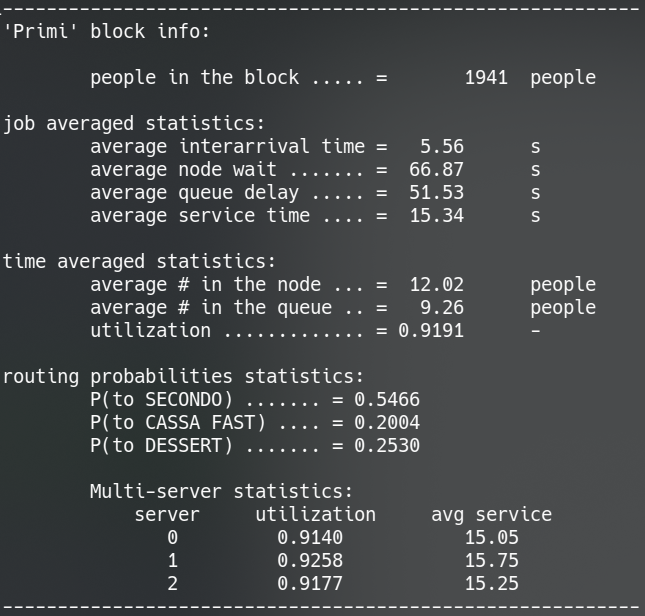
\includegraphics[width=.8\linewidth]{img/primi.png}
  \caption{Centro \textit{PRIMI}.}
  \label{fig:primo}
\end{subfigure}
\begin{subfigure}{.5\textwidth}
  \centering
  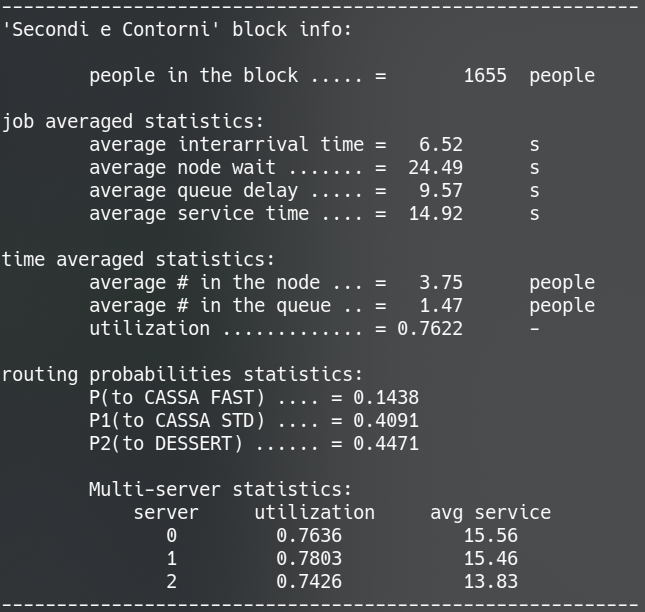
\includegraphics[width=.8\linewidth]{img/secondi.png}
  \caption{Centro \textit{SECONDI}.}
  \label{fig:secondo}
\end{subfigure}
\begin{subfigure}{.5\textwidth}
  \centering
  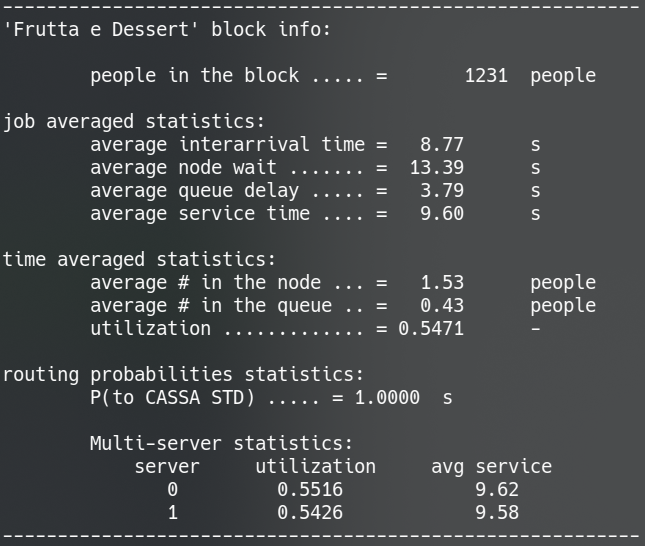
\includegraphics[width=.8\linewidth]{img/dessert.png}
  \caption{Centro \textit{DESSERT}.}
  \label{fig:dessert}
\end{subfigure}%
\begin{subfigure}{.5\textwidth}
  \centering
  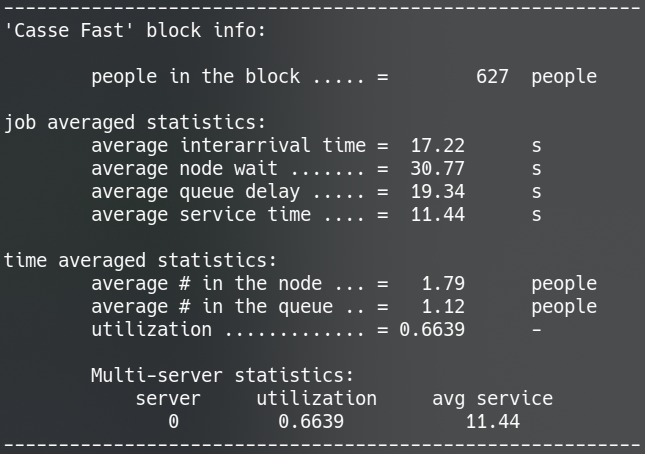
\includegraphics[width=.8\linewidth]{img/cassa_fast.png}
  \caption{Centro \textit{CASSA FAST}.}
  \label{fig:cassa_fast}
\end{subfigure}
\begin{subfigure}{.5\textwidth}
  \centering
  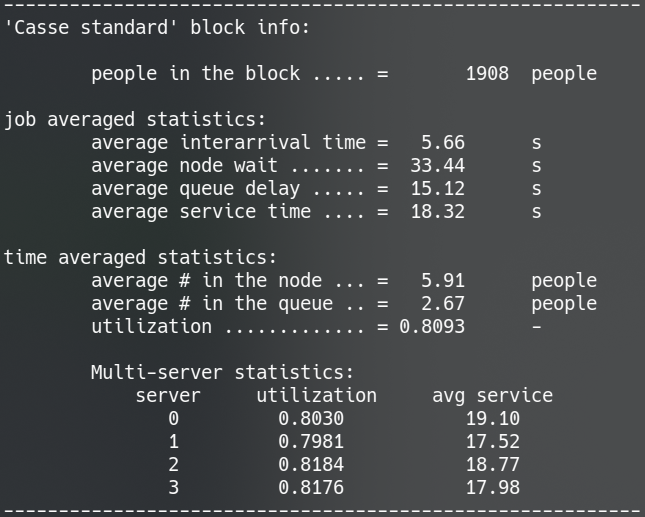
\includegraphics[width=.8\linewidth]{img/cassa_standard.png}
  \caption{Centro \textit{CASSA STD}.}
  \label{fig:cassa_std}
\end{subfigure}
\begin{subfigure}{.5\textwidth}
  \centering
  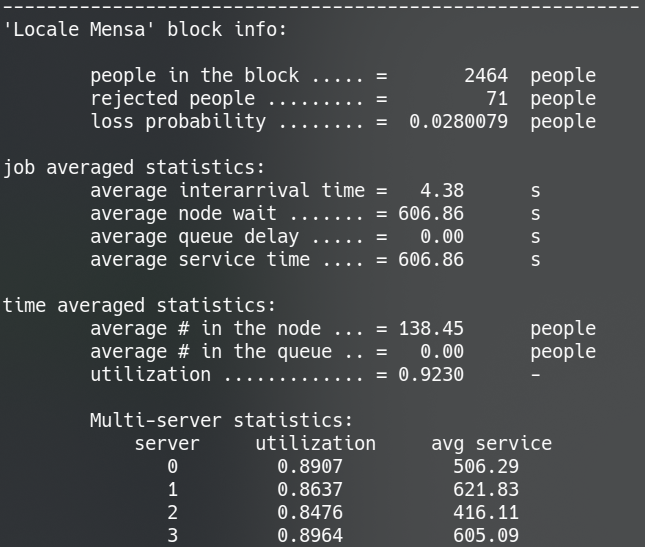
\includegraphics[width=.8\linewidth]{img/consumazione.png}
  \caption{centro \textit{CONSUMAZIONE} (solo i primi 4 posti).}
  \label{fig:consumazione}
\end{subfigure}
\caption{Statistiche di output per ogni centro.}
\label{fig:output}
\end{figure}
\FloatBarrier

\subsection{Controlli di Consistenza}

La prima verifica riguarda la consistenza dei risultati ottenuti per ogni blocco.

\subsubsection{Tempi di risposta nei centri}

Per il tempo medio di risposta in ciascun centro $i$ deve valere: 
\[E(T_{S}) = E(T_{Q}) + E(S)\]
La condizione è verificata per ogni blocco, come mostrato dai tempi simulati riportati in Tab. \ref{tab:tempi_risposta}.

\begin{center}\label{tab:tempi_risposta}
\begin{tabular}{|c|c|c|c|}
 \hline
 \textbf{Centro} & \textbf{$E(T_{Q})$} & \textbf{$E(S)$} & \textbf{$E(T_{S})$}\\
 \hline
 \textit{PRIMO} & \ETqPsim & \ESPsim & \ETSPsim \\
 \hline
 \textit{SECONDO} & \ETqSsim & \ESSsim & \ETSSsim\\
 \hline
 \textit{DESSERT} & \ETqDsim & \ESDsim & \ETSDsim \\
 \hline
 \textit{CASSA FAST} & \ETqFsim & \ESFsim & \ETSFsim \\
 \hline
 \textit{CASSA STD} & \ETqCsim & \ESCsim & \ETSCsim\\
 \hline
 \textit{CONSUMAZIONE} & \ETqLMsim & \ESLMsim & \ETSLMsim \\
 \hline
\end{tabular}
\end{center}

\subsubsection{Popolazioni dei centri}

Un ulteriore controllo di consistenza riguarda il numero di job nel centro pari a: 
\[E(N_{S}) = E(N_{Q}) + m \cdot \rho\]
In Tab. \ref{tab:popolazioni} si può verificare che la formula è soddisfatta.

\begin{center}\label{tab:popolazioni}
\begin{tabular}{|c|c|c|c|c|}
 \hline
 \textbf{Centro} & $E(N_{Q})$ & $m$ & $\rho$ & $E(N_{S})$\\
 \hline
 \textit{PRIMO} & \ENqPsim & \mP & \rhoPsim & \ENsP\\
 \hline
 \textit{SECONDO} & \ENqSsim & \mS & \rhoSsim & \ENsS\\
 \hline
 \textit{DESSERT} & \ENqDsim & \mD & \rhoDsim & \ENsD\\
 \hline
 \textit{CASSA FAST} & \ENqFsim & \mF & \rhoFsim & \ENsF\\
 \hline
 \textit{CASSA STD} & \ENqCsim & \mC & \rhoCsim & \ENsC\\
 \hline
 \textit{CONSUMAZIONE} & \ENqLMsim & \mLM & \rhoLMsim & \ENsLM\\
 \hline
\end{tabular}
\end{center}


%\subsection{Extension Removal}
%Il controllo da eseguire riguarda la variazione nel numero di serventi per un centro. Si vuole verificare che passando da un centro $M/M/m$ ad uno $M/M/1$ l'utilizzazione del blocco sia pari a quella del servente. In Fig. \ref{fig:extension_removal} è riportata la variazione applicata al centro PRIMO, e come entrambi i valori siano pari a $2.6602$.

% \begin{figure}[h]
%   \centering
%   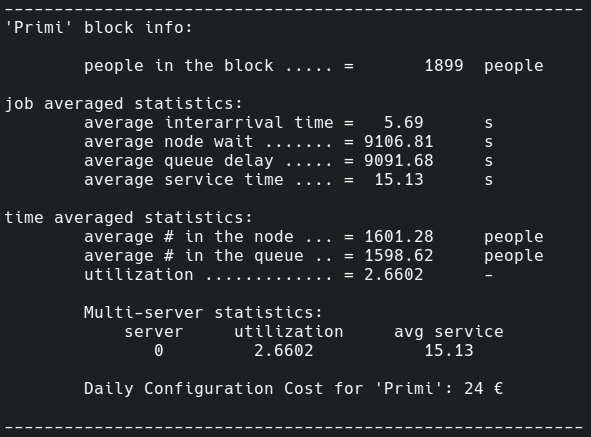
\includegraphics[width=.5\linewidth]{img/extension_removal.png}
%   \caption{Esempio di riduzione del numero di serventi per il centro PRIMI. Notiamo che con un solo servente il centro non è più stabile (\(\rho > 1)\)}
%   \label{fig:extension_removal}
% \end{figure}

\subsection{Dati di Input}

In accordo con quanto definito in Sec. \ref{subsec:dati}, si vuole verificare che i dati computati dalla simulazione riprendano quelli dati in input al sistema.

\subsubsection{Numero Utenti}

Il primo controllo riguarda il numero totale di utenti entrato nel sistema, definito pari a $2500$ in media nel modello delle specifiche, mentre per la simulazione vale $2535$ ottenuto sommando il numero di arrivi per i centri \textit{CASSA FAST} e \textit{CASSA STD} (vedi Fig. \ref{fig:cassa_fast} e Fig. \ref{fig:cassa_std}): $627 + 1908 = 2535$. Se inoltre si verifica il numero di utenti sommando gli utenti accettati e quelli rifiutati nel blocco \textit{CONSUMAZIONE} si ottiene lo stesso risultato: $ 2464 + 71 = 2535 $.
\subsubsection{Tempi e Tassi di Servizio}

Anche i tempi di servizio di ciascun servente riprendono quelli definiti nel modello delle specifiche. In particolare per i tre serventi del centro \textit{PRIMO} (vedi Fig. \ref{fig:primo}) i valori sono $E(S_{P_1}) = 15.05\ s$, $E(S_{P_2}) = 15.75\ s$, $E(S_{P_3}) = 15.25\ s$, dunque vicini al valore di riferimento $E(S_P) = 15\ s$. Inoltre, la media dei tempi restituisce il corrispettivo valore dell'intero blocco: $\frac{15.05 + 15.75 + 15.25}{3} = 15.34\ s$. 

In Tab. \ref{tab:tassi_servizio} sono confrontati i tassi di servizio simulati e quelli passati come input.

\begin{center}\label{tab:tassi_servizio}
\begin{tabular}{|c|c|c|}
 \hline
 \textbf{Centro} & $\mu$ \textbf{Teorico} & $\mu$ \textbf{Simulato}\\
 \hline
 \textit{PRIMO} & \muP & \muPsim\\
 \hline
 \textit{SECONDO} & \muS & \muSsim\\
 \hline
 \textit{DESSERT} & \muD & \muDsim\\
 \hline
 \textit{CASSA FAST} & \muF & \muFsim\\
 \hline
 \textit{CASSA STD} & \muC & \muCsim\\
 \hline
 \textit{CONSUMAZIONE} & \muLM & \muLMsim\\
 \hline
\end{tabular}
\end{center}

Come è possibile vedere, i tassi di servizio simulati sono piuttosto vicini ai valori teorici già con una simulazione di 3 ore.

\subsubsection{Probabilità di Routing}

Sono state verificate anche le probabilità di routing. Ad esempio, considerando il centro \textit{PRIMO} (vedi Fig. \ref{fig:primo}) la probabilità di routing dall'esterno al blocco \textit{PRIMO} è facilmente calcolabile dalla simulazione come la frazione di job entranti nel blocco su quelli totali con la seguente formula:

\begin{center}
\[p_{0, 1} = \frac{job\ uscenti\ da\ PRIMO}{job\ entranti\ da\ esterno}\] 
\end{center}

Il calcolo delle probabilità di routing è eseguito nella funzione \texttt{simulation\_routing\_probabilities\_test()} del file \texttt{analytic\_test.c}. 

In Tab. \ref{tab:servizio} sono presentati i risultati. Anche in questo caso i valori simulati sono in linea con i valori teorici.

\begin{center}\label{tab:servizio}
\begin{tabular}{|c|c|c|c|}
 \hline
 \textbf{Sorgente $i$} & \textbf{Destinazione $j$} & \textbf{\(p_{ij}\) Teorica} & \textbf{\(p_{ij}\) Simulata}\\
 \hline
 \textit{ESTERNO} & \textit{PRIMO}   & \pEP & 0.7656\\
 \hline
 \textit{ESTERNO} & \textit{SECONDO}   & \pES & 0.2343\\
 \hline
 \textit{PRIMO} & \textit{SECONDO}   & \pPS & 0.5466\\
 \hline
 \textit{PRIMO} & \textit{DESSERT}   & \pPD & 0.2530\\
 \hline
 \textit{PRIMO} & \textit{CASSA FAST}   & \pPF & 0.2004\\
\hline
 \textit{SECONDO} & \textit{DESSERT}   & \pSD & 0.4471\\
 \hline
 \textit{SECONDO} & \textit{CASSA FAST}   & \pSF & 0.1438\\
\hline
 \textit{SECONDO} & \textit{CASSA STD}   & \pSC & 0.4091\\
\hline
 \textit{DESSERT} & \textit{CASSA STD}   & \pDC & 1.0000\\
 \hline
 \textit{CASSA FAST} & \textit{CONSUMAZIONE}   & \pFLM & 1.0000\\
 \hline
 \textit{CASSA STD} & \textit{CONSUMAZIONE}   & \pCLM & 1.0000\\
 \hline
 %\textit{CONSUMAZIONE} & \textit{ESTERNO}   & \pLME & \textit{1.0}\\
 %\hline
\end{tabular}
\end{center}


\subsubsection{Tassi di Arrivo}\label{subsub:tassi}
I tassi di arrivo per i centri teorici e simulati (dagli inversi dei tempi di interarrivo) sono i visibili in Tab. \ref{tab:tassi_arrivo}. I tassi di arrivo simulati sono stati ottenuti dall'inverso del tempo di interarrivo medio ottenuto in output da ciascun blocco.
Il tasso di arrivo del blocco \textit{CONSUMAZIONE} considera solamente gli utenti accettati e non quelli rifiutati.
\begin{center}\label{tab:tassi_arrivo}
\begin{tabular}{|c|c|c|}
 \hline
 \textbf{Centro} & $\lambda$ \textbf{Teorico} & $\lambda$ \textbf{Simulato}\\
 \hline
 \textit{PRIMO} & \lambdaP & \LambdaPsim\\
 \hline
 \textit{SECONDO} & \lambdaS & \LambdaSsim\\
 \hline
 \textit{DESSERT} & \lambdaD & \LambdaDsim\\
 \hline
 \textit{CASSA FAST} & \lambdaF & \LambdaFsim\\
 \hline
 \textit{CASSA STD} & \lambdaC & \LambdaCsim\\
 \hline
 \textit{CONSUMAZIONE} & \lambdaLM & \LambdaLMsim\\
 \hline
\end{tabular}
\end{center}

\subsubsection{Visite medie}

Abbiamo verificato le visite medie rispetto a quelle teoriche. Sappiamo che la formula per il calcolo delle visite medie in una rete aperta è la seguente:
\[v_i = \frac{\lambda_i}{\lambda} \]
In Tab. \ref{tab:visite} è possibile osservare come i valori simulati delle visite sono perlopiù vicini a quelli teorici, già con una simulazione di sole 3 ore\footnote{Le visite (e i tassi di arrivo) per il blocco \textit{CONSUMAZIONE} sono calcolate con usando $\lambda^{'}=\lambda \cdot (1 - p_{loss})$.}. Per i dettagli sull'implementazione, si rimanda alla funzione \texttt{simulation\_visit\_test()} del file \texttt{analytic\_test.c}.

\begin{center}\label{tab:visite}
\begin{tabular}{|c|c|c|}
 \hline
 \textbf{Centro} & $v_i$ \textbf{Teorico} & $v_i$ \textbf{Simulato}\\
 \hline
 \textit{PRIMO} & \vP & \vPsim \\
 \hline
 \textit{SECONDO} & \vS & \vSsim \\
 \hline
 \textit{DESSERT} & \vD & \vDsim \\
 \hline
 \textit{CASSA FAST} & \vF & \vFsim \\
 \hline
 \textit{CASSA STD} & \vC & \vCsim \\
 \hline
 \textit{CONSUMAZIONE} & \vLM & \vLMsim \\
 \hline
\end{tabular}
\end{center}

\subsubsection{Utilizzazioni}

In Tab. \ref{tab:rho} è possibile osservare come i valori simulati si avvicinano ai valori teorici.

\begin{center}\label{tab:rho}
\begin{tabular}{|c|c|c|}
 \hline
 \textbf{Centro} & $\rho$ \textbf{Teorica} & $\rho$ \textbf{Simulata}\\
 \hline
 \textit{PRIMO} & \rhoP & \rhoPsim\\
 \hline
 \textit{SECONDO} & \rhoS & \rhoSsim\\
 \hline
 \textit{DESSERT} & \rhoD & \rhoDsim\\
 \hline
 \textit{CASSA FAST} & \rhoF & \rhoFsim\\
 \hline
 \textit{CASSA STD} & \rhoC & \rhoCsim\\
 \hline
 \textit{CONSUMAZIONE} & \rhoLM & \rhoLMsim\\
 \hline
\end{tabular}
\end{center}
Se si aumenta il numero di ore di simulazione, si può verificare che le utilizzazioni simulate tendono alle simulazioni teoriche.
Per i dettagli sull'implementazione, si faccia riferimento alla funzione \texttt{get\_stats()} nel file \texttt{helpers.c}.

\subsection{QoS}

Vengono ora confrontati i QoS della simulazione con quelli calcolati usando le formule teoriche e i dati nel modello delle specifiche.

\subsubsection{Tempo di Risposta Globale}
E' necessario verificare anche il tempo di risposta globale, che si ricorda essere un QoS. 

Sia $v_{i}$ il numero di visite medie nel centro $i$ nella nostra rete aperta ed $E(T_{r, i})$ il tempo di risposta del centro $i$. Il tempo di risposta globale teorico della rete è calcolato come segue:
\[E(T_{r}^{(t)}) = \sum_{i=1}^{M} E(T_{S,i})^{(t)} \cdot v_{i}^{(t)} = \ETSglobale\ s\] 

Il risultato simulato è invece: 
\[E(T_{r}^{(s)}) =  \sum_{i=1}^{M} E(T_{S,i})^{(s)} \cdot v_{i}^{(s)} = \ETSglobaleSim\ s\]

I due risultati non coincidono ma, come vedremo nella simulazione a orizzonte infinito, all'aumentare del tempo di simulazione il tempo di risposta globale simulato tende a quello teorico.
\subsubsection{Probabilità di Perdita}

Il secondo QoS riguarda il solo centro \textit{CONSUMAZIONE}. 
Con 150 posti a sedere la probabilità di perdita è la seguente:

\[p_{loss}^{(t)}=\frac{\frac{1}{m!} \cdot (\frac{\lambda}{\mu})^m}{\sum_{j=0}^{m}{\frac{1}{j!} \cdot (\frac{\lambda}{\mu})^j}} = 0.0251 \]
La probabilità simulata è:
\[p_{loss}^{(s)}=0.0280\]

Si ottiene dunque $p_{loss}^{(s)} > p_{loss}^{(t)}$, ma a fronte di numero di ore per la simulazione molto basso. Nel seguito vedremo che questo valore si avvicinerà di più a quello teorico.

\section{Validazione}

Il sistema in analisi è ipotetico, dunque non prende uno specifico modello reale come riferimento. Non è dunque possibile validarlo confrontando i risultati del modello computazionale con i risultati del sistema reale. 

Il processo di validazione si riconduce quindi a studiare il comportamento del modello con piccole variazioni al tasso di arrivo.

\subsection{Aumento del Tasso di Arrivo}

Aumentando il tasso di arrivo a $\lambda = 0.25 \frac{arrivi}{secondo}$ si osserva una maggiore probabilità di perdita, ma una diminuzione del tempo di risposta.  

I valori sono riportati in Tab. \ref{tab:tempo_risposta_aumentato} e \ref{tab:p_loss_aumentato}\footnote{Nel transiente si fa riferimento a 250 repliche.}.

\subsubsection{Tempo di Risposta Globale}

\begin{center}\label{tab:tempo_risposta_aumentato}
\begin{tabular}{|c|c|}
\hline
\textbf{Statistica} & \textbf{Risultato}\\
 \hline
\(E(T_{r})^{teorico}\) & 695.6529\ s \\
\hline
\(E(T_{r})^{transiente}\) & 695.4047\ s $\pm$ 3.404221\ s\\
\hline
\(E(T_{r})^{stazionario}\) & 696.260618\ s $\pm$ 2.274880\ s\\
 \hline
\end{tabular}
\end{center}

\subsubsection{Probabilità di Perdita}

\begin{center}\label{tab:p_loss_aumentato}
\begin{tabular}{|c|c|}
\hline
\textbf{Statistica} & \textbf{Risultato}\\
 \hline
\(p_{loss}^{teorico}\) & 0.062403 \\
\hline
\(p_{loss}^{transiente}\) & 0.052404 $\pm$ 0.001833 \\
\hline
\(p_{loss}^{stazionario}\) & 0.062450 $\pm$ 0.001089 \\
 \hline
\end{tabular}
\end{center}

\subsection{Diminuzione del Tasso di Arrivo}

Con una diminuzione del tasso di arrivo a $\lambda = 0.2 \frac{arrivi}{secondo}$ si osservano valori più piccoli sia per la probabilità di perdita che nel tempo di risposta.  

I valori simulati sono riportati in Tab. \ref{tab:tempo_risposta_dim} e \ref{tab:p_loss_dim}.

\subsubsection{Tempo di Risposta Globale}

\begin{center}\label{tab:tempo_risposta_dim}
\begin{tabular}{|c|c|}
\hline
\textbf{Statistica} & \textbf{Risultato}\\
 \hline
\(E(T_{r})^{teorico}\) & 663.4007\ s \\
\hline
\(E(T_{r})^{transiente}\) & 664.6840\ s $\pm$ 1.5800\ s\\
\hline
\(E(T_{r})^{stazionario}\) & 662.6915\ s $\pm$ 0.8893\ s\\
 \hline
\end{tabular}
\end{center}

\subsubsection{Probabilità di Perdita}

\begin{center}\label{tab:p_loss_dim}
\begin{tabular}{|c|c|}
\hline
\textbf{Statistica} & \textbf{Risultato}\\
 \hline
\(p_{loss}^{teorico}\) & 0.0010 \\
\hline
\(p_{loss}^{transiente}\) &  0.0008 $\pm$ 0.0002\\
\hline
\(p_{loss}^{stazionario}\) & 0.0009 $\pm$ 0.0001\\
 \hline
\end{tabular}
\end{center}


\section{Processo degli esperimenti}

In questo capitolo sarà presentato e discusso lo studio delle statistiche transienti e stazionarie ottenute nelle simulazioni ad orizzonte temporale finito e infinito.

\subsection{Simulazione Finite-Horizon}

Nella simulazione ad orizzonte temporale finito si è studiato l'andamento del tempo globale di risposta e la probabilità di perdita \textbf{transienti}, sia al variare del numero di repliche che in funzione del seed.

\subsubsection{Variazione del Seed - Simulazione Singola}

Prima di vedere l'andamento delle statistiche di interesse con la replicazione, è interessante vedere l'andamento dei risultati prodotti da \textbf{singole simulazioni} di diversa durata, facendo variare il seed del sistema, per verificare il suo comportamento.

In Fig. \ref{fig:grt_seed_finite} e Fig. \ref{fig:ploss_seed_finite} è mostrato come per all'\textbf{aumentare del periodo di osservazione} i risultati ottenuti hanno un andamento asintotico, ma distante dal valore teoruco; inoltre ma c'è una grande varianza tra gli andamenti dei diversi seed. In particolare, in Fig. \ref{fig:grt_seed_finite} i tempi tendono ad avvicinarsi al tempo di risposta teorico, mentre in Fig. \ref{fig:ploss_seed_finite} la differenza con il valore di riferimento è maggiore, ma anche la scala del grafico risulta essere a grana molto fine. E' quindi necessario procedere con la simulazione finite-horizon basata su replicazione, per ridurre la varianza di questi risultati transienti.

\begin{figure}[htbp]
  \centering
  \includesvg[inkscapelatex=false, width = 370pt]{grt_seed_finite.svg}
  \caption{Andamento del tempo globale di risposta al variare del seed di sistema.}
  \label{fig:grt_seed_finite}
\end{figure}

\begin{figure}[htbp]
  \centering
  \includesvg[inkscapelatex=false, width = 370pt]{ploss_seed_finite.svg}
  \caption{Andamento della probabilità di perdita al variare del seed di sistema.}
  \label{fig:ploss_seed_finite}
\end{figure}
\FloatBarrier

\subsubsection{Replicazione}

In questa analisi si è variato il numero di repliche per ciascun \textbf{ensemble} partendo da un insieme di 50 fino a 500, con incrementi di 50 repliche ad ogni iterazione. 

Gli stream sono inizializzati una sola volta invocando \texttt{PlantSeed()} prima del ciclo di replicazione, mentre tra una simulazione e la successiva si riutilizza lo stato finale di ogni stream. In questo modo è possibile generare \textbf{stime indipendenti} della stessa statistica \textbf{transiente}.

La condizione di terminazione è sempre il tempo \textit{close-the-doors}, ovvero una durata complessiva di 3 ore, e inoltre il numero di job in ogni blocco all'inizio e alla fine è zero.

Per ogni ensemble vengono calcolate, con l'algoritmo \textbf{one-pass di Wellford}, \textbf{media} e \textbf{deviazione standard} e quindi l'intervallo di confidenza al $95\ \%$. Il calcolo degli intervalli è stato implementato sulla base del file \texttt{estimate.c}. 

Con i risultati ottenuti si vuole dimostrare come all'aumentare del numero di simulazioni, i valori medi tendono a un certo valore diverso da quello teorico, che rappresenta la media della statistica transiente. Inoltre, è possibile notare che all'aumentare delle replicazioni, l'intervallo di confidenza ha un'ampiezza sempre più piccola. 

% In Fig. \ref{fig:grt_finite_replicas} e Fig. \ref{fig:ploss_finite_replicas} è mostrato come da un certo numero di repliche (i.e., $\simeq 300$) l'ampiezza gli intervalli per entrambe le statistiche rimanga costante e inferiore rispetto agli ensemble precedenti.
% E' possibile osservare come il valore del tempo globale di risposta sia compreso nella maggior parte degli intervalli rappresentati. Il discorso non è analogo per la probabilità di perdita. Infatti, per quest'ultima nessun intervallo la contiene. Ciò è dovuto ai valori molto piccoli che si stanno considerando. 
Nelle Fig. \ref{fig:grt_finite_replicas} e Fig. \ref{fig:ploss_finite_replicas} si può notare come i valori transienti si discostino dai valori teorici stazionari. Poiché il tempo di simulazione di 3 ore è troppo basso per portare a regime il blocco \textit{CONSUMAZIONE}, c'è una forte \textbf{dipendenza dalle condizioni iniziali}, che rende il tempo di risposta maggiore (perché molti trovano posto e rimangono a mangiare) e la probabilità di perdita minore (perché la mensa inizialmente è vuota). Questo è di \textbf{grande interesse} per l'analisi in quanto questa situazione si presenterebbe ogni giorno in un ipotetico sistema reale organizzato secondo questo modello. Con 10.000 repliche, il tempo di risposta transiente è \(674.642288 \pm 0.241640\) s (superiore di 1.5 s rispetto allo stazionario), mentre la probabilità di perdita è \(0.020559 \pm 0.000211\) (inferiore di 0.5 punti percentuali rispetto alla probabilità di perdita stazionaria).

Quindi è di maggiore interesse la simulazione a orizzonte finito rispetto a quella a orizzonte infinito, perché permette di avere una visione del modello molto più vicina a quella reale.

\begin{figure}[htbp]
  \centering
  \includesvg[inkscapelatex=false, width = 370pt]{grt_finite_replicas.svg}
  \caption{Andamento del tempo globale di risposta all'aumentare del numero di repliche.}
  \label{fig:grt_finite_replicas}
\end{figure}

\begin{figure}[htbp]
  \centering
  \includesvg[inkscapelatex=false, width = 370pt]{ploss_finite_replicas.svg}
  \caption{Andamento della probabilità di perdita all'aumentare del numero di repliche.}
  \label{fig:ploss_finite_replicas}
\end{figure}
\FloatBarrier
\subsection{Simulazione Infinite-Horizon}

L'obiettivo è studiare l'andamento del sistema in un tempo molto più grande di quello operativo (i.e., 3 ore). 

\subsubsection{Batch Means}

Il primo passo nell'utilizzo dell'algoritmo batch means è la scelta dei parametri \textit{b} (dimensione del batch) ed \textit{n} (numero di job), per poter cosi ricavare il numero di job appartenenti ad ogni batch. Per prima cosa è stato fissato il numero di utenti totali a un numero molto grande:
\[n = 2.5 \cdot 10^6\]
Dopodiché, per scegliere il numero di batch tenendo fisso il numero di utenti, sono state seguite le linee guida del libro\footnote{\textit{Leemis L. M. \& Park S. K. (2006). Discrete-event simulation : a first course. Pearson Prentice Hall.}}. In particolare il criterio considerato per la scelta del numero di batch è basato sul calcolo dell'\textbf{autocorrelazione}\footnote{\textit{Banks, Carson, Nelson, and Nicol (2001, page 483).}}, che deve essere inferiore a 0.2 in corrispondenza di un lag pari a 1. Per il calcolo delle autocorrelazioni ci si è basati sul programma \texttt{acs.c}, che è stato integrato nel codice della simulazione batch means. Quindi, una volta implementato il codice relativo alla simulazione a orizzonte infinito, sono stati fatti diversi tentativi nella scelta di \(b\), finché l'autocorrelazione per tempo di risposta e probabilità di perdita fosse minore di 0.2. I parametri adottati sono dunque: 

\[b = 2000\]

\[k = \floor*{\frac{n}{b}} = \floor*{\frac{2.5 \cdot 10^{6}}{2 \cdot 10^{3}}} = 1250\]

In Fig. \ref{fig:auto_grt} e Fig. \ref{fig:auto_ploss} sono riportati i valori delle autocorrelazioni. 

Dopodiché viene eseguita una lunga simulazione di \(n\) job, in cui ad ogni \(b\) job vengono calcolati i tempi di risposta e le probabilità di perdita del batch. A questo punto lo stato del sistema (numero di job in coda e job nel centro) viene lasciato invariato\footnote{In quanto nella simulazione a orizzonte infinito non è di interesse che il sistema torni allo stato iniziale.}, si azzerano le sole statistiche di output (e.g., tempi di risposta, aree, job completati) e in questo modo è possibile calcolare i tempi di risposta e le probabilità di perdita solo in base ai valori del batch, e non dall'inizio, a differenza di come fatto per la simulazione a orizzonte finito. Grazie a questo accorgimento le medie dei batch sono indipendenti tra loro.

Al termine della simulazione a orizzonte finito, vengono calcolate le medie e le deviazioni standard delle medie dei batch per tempo di risposta e probabilità di perdita, così da costruire un intervallo di confidenza.

\begin{figure}[h]
\begin{subfigure}{.5\textwidth}
  \centering
  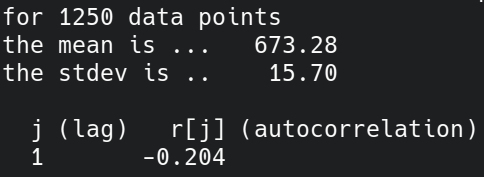
\includegraphics[width=.75\linewidth]{img/auto_grt.png}
  \caption{Tempo di risposta globale.}
  \label{fig:auto_grt}
\end{subfigure}%
\begin{subfigure}{.5\textwidth}
  \centering
  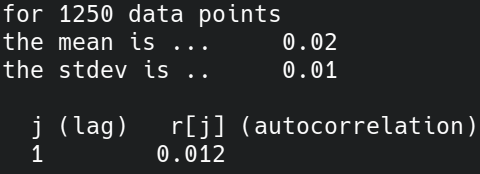
\includegraphics[width=.75\linewidth]{img/auto_ploss.png}
  \caption{Probabilità di perdita.}
  \label{fig:auto_ploss}
\end{subfigure}
\caption{Autocorrelazione per il tempo medio di risposta globale e la probabilità di perdita.}
\label{fig:output_autocorrelazione}
\end{figure}
\FloatBarrier

In Fig. \ref{fig:grt_infinite_batch} è possibile osservare come si raggiunga la stazionarietà del tempo di risposta globale già al 300esimo batch, che corrisponde a 600.000 arrivi nella mensa. 

Per quanto riguarda la probabilità di perdita (vedi Fig. \ref{fig:ploss_infinite_batch}) i valori raggiungo la stazionarietà all'incirca dall'800esimo batch. In questo caso, la maggiore distanza tra valore teorico e simulato è dovuta ad una scala più grande dei valori rappresentati. 

\begin{figure}[htbp]
  \centering
  \includesvg[inkscapelatex=false, width = 370pt]{grt_infinite_batch.svg}
  \caption{Andamento del tempo globale di risposta medio all'aumentare del numero di batch.}
  \label{fig:grt_infinite_batch}
\end{figure}

\begin{figure}[htbp]
  \centering
  \includesvg[inkscapelatex=false, width = 370pt]{ploss_infinite_batch.svg}
  \caption{Andamento della probabilità di perdita media all'aumentare del numero di batch.}
  \label{fig:ploss_infinite_batch}
\end{figure}
\FloatBarrier

\subsubsection{Consistenza sul Batch Means}

Per controllare la correttezza dei risultati ottenuti si è confrontata la media risultante dai batch con quella ottenuta da un'unica simulazione della stessa durata. In Tab. \ref{tab:batch} si può osservare quanto i risultati siano vicini tra loro.

\begin{center}\label{tab:batch}
\begin{tabular}{|c|c|c|c|}
 \hline
 \textbf{$E(T_{r})^{batch}$} & \textbf{$E(T_{r})^{singolo\ run}$} & \textbf{$p_{loss}^{batch}$} & \textbf{$p_{loss}^{singolo\ run}$}\\
 \hline
 673.278713 s & 673.009476 s & 0.024949 & 0.024958\\
 \hline
\end{tabular}
\end{center}

\subsubsection{Variazione del Seed}

Come nella simulazione finita, si è voluto studiare un'eventuale variazione dei risultati tra seed diversi nel batch means. 

In Fig. \ref{fig:grt_seed_infinite} e Fig. \ref{fig:ploss_seed_infinite} si nota come le medie siano molto simili tra loro e tutte prossime ai valori teorici sia per il tempo di risposta che per la probabilità di perdita. 

\begin{figure}[htbp]
  \centering
  \includesvg[inkscapelatex=false, width = 370pt]{grt_seed_infinite.svg}
  \caption{Intervalli di confidenza per il tempo globale di risposta al variare del seed di sistema.}
  \label{fig:grt_seed_infinite}
\end{figure}

\begin{figure}[htbp]
  \centering
  \includesvg[inkscapelatex=false, width = 370pt]{ploss_seed_infinite.svg}
  \caption{Intervalli di confidenza per la probabilità di perdita al variare del seed di sistema.}
  \label{fig:ploss_seed_infinite}
\end{figure}
\FloatBarrier

\section{Modello Migliorativo}

Alla luce dei risultati conseguiti nel modello presentato fino ad ora, in questo capitolo vengono proposte tre varianti della zona \textit{CONSUMAZIONE} con l'obiettivo di annullare il numero di dipendenti che non trovano un posto a sedere.

La prima miglioria considerata è di aumentare il numero di posti a sedere passando dai 150 iniziali a 200. In Fig. \ref{fig:esteso_1_concettuale} è riportato il modello concettuale aggiornato\footnote{Le zone \textit{Ristorazione} e \textit{Casse} sono invariate rispetto al modello base.}.

\begin{figure}[H]
\centering
 \includesvg[width=.75\linewidth]{esteso_1.svg}
 \caption{Modello concettuale migliorativo con aumento dei posti a sedere.}
  \label{fig:esteso_1_concettuale}
\end{figure}
\FloatBarrier

Ne segue che il \textbf{modello delle specifiche} e il \textbf{modello computazionale} è pressocché invariato rispetto a quanto discusso in Sec. \ref{sec:specifiche} e Sec. \ref{sec:computazionale}.

\subsection{Verifica}

I dati ottenuti fanno riferimento ad una singola simulazione con durata pari al periodo di osservazione (i.e.,  3 ore) e seed pari a 123456789 (vedi Fig. \ref{fig:output_ext_1}).

\begin{figure}[H]
\begin{subfigure}{.5\textwidth}
  \centering
  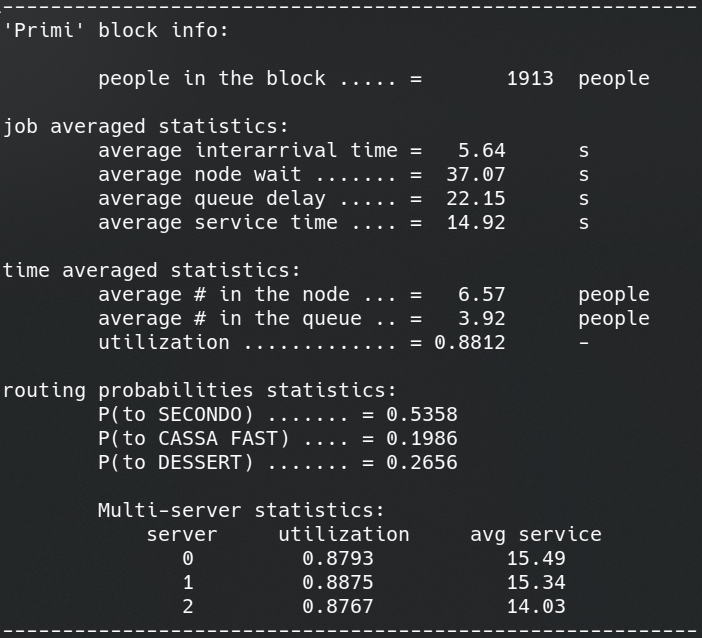
\includegraphics[width=.9\linewidth]{img/migliorativo_1/primo_ext_1.png}
  \caption{Centro PRIMI.}
  \label{fig:primo_ext_1}
\end{subfigure}
\begin{subfigure}{.5\textwidth}
  \centering
  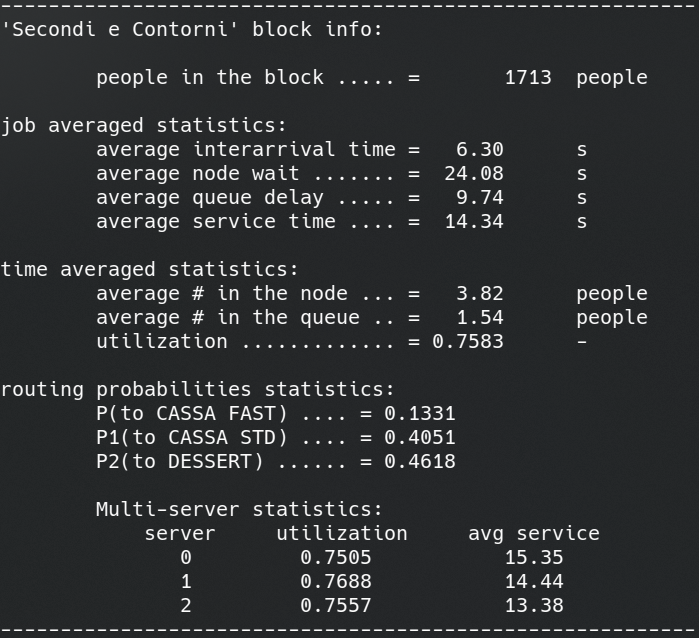
\includegraphics[width=.94\linewidth]{img/migliorativo_1/secondo_ext_1.png}
  \caption{Centro SECONDI.}
  \label{fig:secondo_ext_1}
\end{subfigure}
\begin{subfigure}{.5\textwidth}
  \centering
  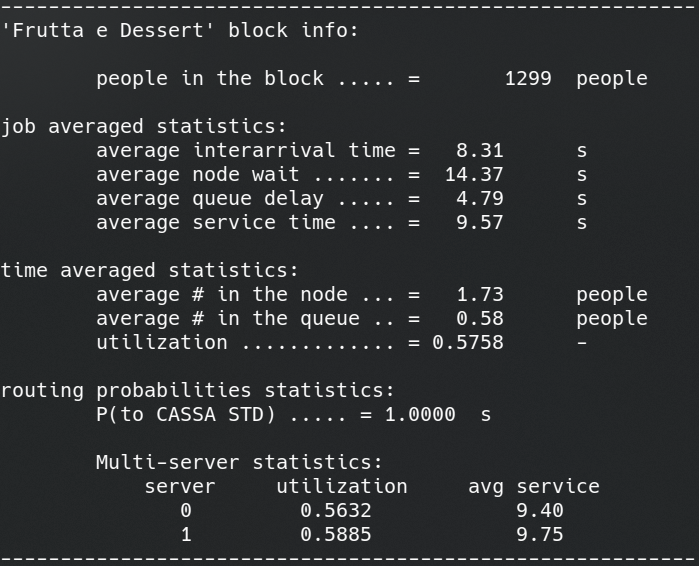
\includegraphics[width=.9\linewidth]{img/migliorativo_1/dessert_ext_1.png}
  \caption{Centro DESSERT.}
  \label{fig:dessert_ext_1}
\end{subfigure}
\begin{subfigure}{.5\textwidth}
  \centering
  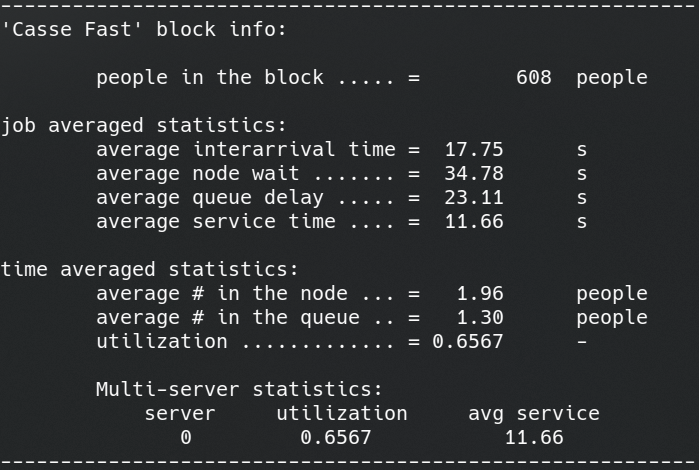
\includegraphics[width=.88\linewidth]{img/migliorativo_1/fast_ext_1.png}
  \caption{Centro CASSA FAST.}
  \label{fig:cassa_fast_ext_1}
\end{subfigure}
\begin{subfigure}{.5\textwidth}
  \centering
  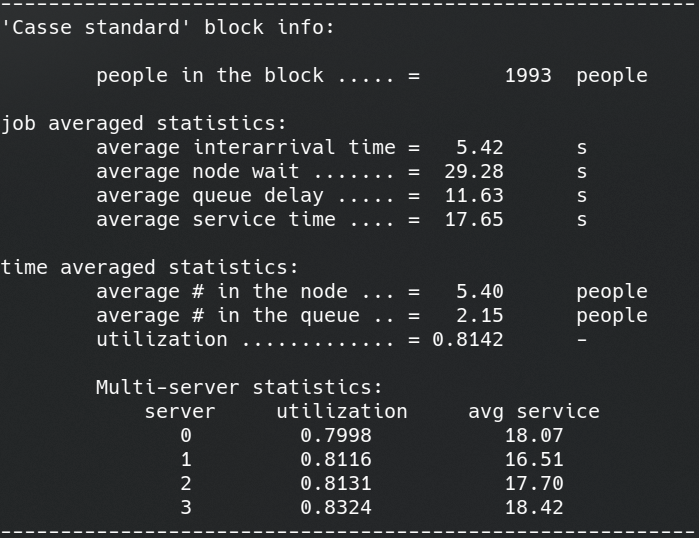
\includegraphics[width=.9\linewidth]{img/migliorativo_1/standard_ext_1.png}
  \caption{Centro CASSA STD.}
  \label{fig:cassa_std_ext_1}
\end{subfigure}
\begin{subfigure}{.5\textwidth}
  \centering
  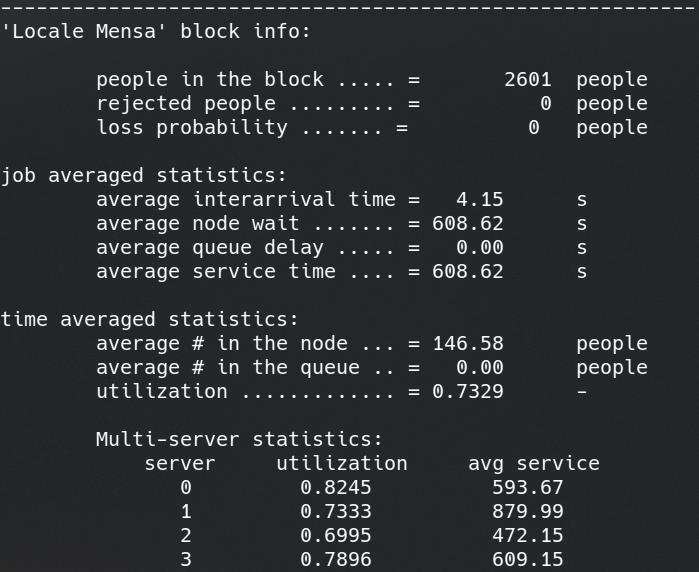
\includegraphics[width=.9\linewidth]{img/migliorativo_1/consumazione_ext_1.png}
  \caption{centro CONSUMAZIONE (solo i primi 4 posti).}
  \label{fig:consumazione_ext_1}
\end{subfigure}
\caption{Statistiche di output per ogni centro.}
\label{fig:output_ext_1}
\end{figure}

\subsubsection{Controlli di Consistenza}

Per i \textbf{tempi di risposta} nei centri le condizioni continuano ad essere verificate per ogni blocco, come mostrato in tabella:
\begin{center}
\begin{tabular}{|c|c|c|c|}
 \hline
 \textbf{Centro} & \textbf{$E(T_{Q})$} & \textbf{$E(S)$} & \textbf{$E(T_{r})$}\\
 \hline
 \textit{PRIMO} & 22.15 & 14.92 & 37.07 \\
 \hline
 \textit{SECONDO} & 9.74 & 14.34 & 24.08\\
 \hline
 \textit{DESSERT} & 4.79 & 9.57 & 14.37\\
 \hline
 \textit{CASSA FAST} & 23.11 & 11.66 & 34.78\\
 \hline
 \textit{CASSA STD} & 11.63 & 17.65 & 29.28\\
 \hline
 \textit{CONSUMAZIONE} & 0 & 608.62 & 608.62\\
 \hline
\end{tabular}
\end{center}
Cosi come le \textbf{popolazioni} dei centri:
\begin{center}\label{tab:popolazioni_ext_1}
\begin{tabular}{|c|c|c|c|c|}
 \hline
 \textbf{Centro} & $E(N_{Q})$ & $m$ & $\rho$ & $E(N_{S})$\\
 \hline
 \textit{PRIMO} & 3.92 & \mP & 0.8812 & 6.57\\
 \hline
 \textit{SECONDO} & 1.54 & \mS & 0.7583 & 3.82\\
 \hline
 \textit{DESSERT} & 0.58 & \mD & 0.5758 & 1.73\\
 \hline
 \textit{CASSA FAST} & 1.30 & \mF & 0.6567 & 1.96\\
 \hline
 \textit{CASSA STD} & 2.15 & \mC & 0.8142 & 5.40\\
 \hline
 \textit{CONSUMAZIONE} & 0 & 200 & 0.7329 & 146.58\\
 \hline
\end{tabular}
\end{center}

\subsection{Dati di Input}

Il \textbf{numero di utenti}  nel sistema con 200 posti in \textit{CONSUMAZIONE} vale $2601$ ottenuto sommando il numero di arrivi nelle casse (vedi Fig. \ref{fig:cassa_fast_ext_1} e Fig. \ref{fig:cassa_std_ext_1}) oppure nel blocco consumazione:

\[E(N_F)+E(N_C) = 608 + 1993 = 2601 = E(N_S)\]

Considerando i \textbf{tempi di servizio} dei soli tre serventi del centro \textit{PRIMO} (vedi Fig. \ref{fig:primo_ext_1}) si ottiene $E(S_{1}) = 15.49\ s$, $E(S_{2}) = 15.34\ s$, $E(S_{3}) = 14.03\ s$, dunque vicini al valore di riferimento $E(S) = 15\ s$. Inoltre, la media dei tempi restituisce il corrispettivo valore dell'intero blocco: $\frac{15.49 + 15.34 + 14.03}{3} = 14.92\ s$. Nella tabella che segue sono confrontati i \textbf{tassi di servizio} simulati e quelli passati come input.
\begin{center}\label{tab:tassi_servizio_ext_1}
\begin{tabular}{|c|c|c|}
 \hline
 \textbf{Centro} & $\mu$ \textbf{Teorico} & $\mu$ \textbf{Simulato}\\
 \hline
 \textit{PRIMO} & \muP & 0.06702\\
 \hline
 \textit{SECONDO} & \muS & 0.069735\\
 \hline
 \textit{DESSERT} & \muD & 0.104493 \\
 \hline
 \textit{CASSA FAST} & \muF & 0.085763\\
 \hline
 \textit{CASSA STD} & \muC & 0.056657 \\
 \hline
 \textit{CONSUMAZIONE} & \muLM & 0.001643\\
 \hline
\end{tabular}
\end{center}

I risultati per le \textbf{probablità di routing} sono:
\begin{center}\label{tab:routing_ext_1}
\begin{tabular}{|c|c|c|c|}
 \hline
 \textbf{Sorgente $i$} & \textbf{Destinazione $j$} & \textbf{\(p_{ij}\) Teorica} & \textbf{\(p_{ij}\) Simulata}\\
 \hline
 \textit{ESTERNO} & \textit{PRIMO}   & 0.7500 & 0.735486 \\
 \hline
 \textit{ESTERNO} & \textit{SECONDO}   & 0.2500 & 0.264514\\
 \hline
 \textit{PRIMO} & \textit{SECONDO}   & 0.5500 & 0.535808\\
 \hline
 \textit{PRIMO} & \textit{DESSERT}   & 0.2500 & 0.265551\\
 \hline
 \textit{PRIMO} & \textit{CASSA FAST}   & 0.2000 & 0.198641\\
\hline
 \textit{SECONDO} & \textit{DESSERT}   & 0.4500 & 0.461763\\
 \hline
 \textit{SECONDO} & \textit{CASSA FAST}   & 0.1375 & 0.1331\\
\hline
 \textit{SECONDO} & \textit{CASSA STD}   & 0.4125 & 0.405137\\
\hline
 \textit{DESSERT} & \textit{CASSA STD}   & 1.0000 & 1.00000\\
 \hline
 \textit{CASSA FAST} & \textit{CONSUMAZIONE}   & 1.0000 & 1.0000\\
 \hline
 \textit{CASSA STD} & \textit{CONSUMAZIONE}   & 1.0000 & 1.0000\\
 \hline
\end{tabular}
\end{center}
I \textbf{tassi di arrivo} simulati e teorici sono calcolati con lo stesso sistema presentato in Sec. \ref{subsub:tassi} e pari a: 
\begin{center}\label{tab:tassi_arrivo_ext_1}
\begin{tabular}{|c|c|c|}
 \hline
 \textbf{Centro} & $\lambda$ \textbf{Teorico} & $\lambda$ \textbf{Simulato}\\
 \hline
 \textit{PRIMO} & 0.1735 & 0.1770\\
 \hline
 \textit{SECONDO} & 0.1534 & 0.1585\\
 \hline
 \textit{DESSERT} & 0.1124 & 0.1202\\
 \hline
 \textit{CASSA FAST} & 0.0558 & 0.0562\\
 \hline
 \textit{CASSA STD} & 0.1757 & 0.1844\\
 \hline
 \textit{CONSUMAZIONE} & 0.2315 & 0.2404\\
 \hline
\end{tabular}
\end{center}
Mentre per le \textbf{visite medie} si ha:
\begin{center}\label{tab:visite_ext_1}
\begin{tabular}{|c|c|c|}
 \hline
 \textbf{Centro} & $v_i$ \textbf{Teorico} & $v_i$ \textbf{Simulato}\\
 \hline
 \textit{PRIMO} & 0.7500 & 0.735486\\
 \hline
 \textit{SECONDO} & 0.6625 & 0.658208\\
 \hline
 \textit{DESSERT} & 0.4856 & 0.499423\\
 \hline
 \textit{CASSA FAST} & 0.2410 & 0.233756\\
 \hline
 \textit{CASSA STD} & 0.7589 & 0.766244\\
 \hline
 \textit{CONSUMAZIONE} & 1.0000 & 1.0000\\
 \hline
\end{tabular}
\end{center}

Le \textbf{utilizzazioni} ottenute sono:
\begin{center}\label{tab:rho_ext_1}
\begin{tabular}{|c|c|c|}
 \hline
 \textbf{Centro} & $\rho$ \textbf{Teorica} & $\rho$ \textbf{Simulata}\\
 \hline
 \textit{PRIMO} & 0.8677 & 0.8812\\
 \hline
 \textit{SECONDO} & 0.7670 & 0.7583\\
 \hline
 \textit{DESSERT} & 0.5620 & 0.5758\\
 \hline
 \textit{CASSA FAST} & 0.6138 & 0.6567\\
 \hline
 \textit{CASSA STD} & 0.7906 & 0.8142\\
 \hline
 \textit{CONSUMAZIONE} & 0.6945 & 0.7329\\
 \hline
\end{tabular}
\end{center}

\subsection{QoS}

Per il \textbf{tempo di risposta globale} si ha: 
\[E(T_{r}^{(t)}) = \sum_{i=1}^{M} E(T_{S,i}) \cdot v_{i} \]
\[= E(T_{S,1}) \cdot v_1+ E(T_{S,2}) \cdot v_{2} + E(T_{S,3}) \cdot v_{3} + E(T_{S,F}) \cdot v_{F} + E(T_{S,C}) \cdot v_{C} + E(T_{S,S}) \cdot v_{S}\]
\[=  43.8488 \cdot 0.75 + 27.7345 \cdot 0.6625 + 14.6181 \cdot 0.4856 + 28.4897 \cdot 0.2410 + 30.4488 \cdot 0.7589 + 600 \cdot 1\]
\[ = 688.3362\ s\]
Per il simulato: 
\[E(T_{r}^{(s)}) = 689.4784\ s\]
Infine, con 200 posti a sedere la \textbf{probabilità di perdita} è:
\[p_{loss}^{(t)} \simeq p_{loss}^{(s)} = 0 \]

\section{Modello Migliorativo 2 con Politica Random}\label{sec:migliorativo_2_random}

La seconda proposta per il blocco \textit{CONSUMAZIONE} considera la possibilità di avere due zone separate dove poter pranzare, ma di dimensione ridotta rispetto al caso precedente. Quest'idea nasce come alternativa all'ampliamento dello spazio già presente. Dunque si usa una zona aggiuntiva, separata da quella iniziale.
In Fig. \ref{fig:esteso_2_concettuale} è presentato il modello concettuale con 100 posti per ciascuna zona.

\begin{figure}[H]
\centering
 \includesvg[width=.65\linewidth]{esteso_2.svg}
  \caption{Modello concettuale migliorativo con aggiunta del blocco \textit{CONSUMAZIONE 2}.}
  \label{fig:esteso_2_concettuale}
\end{figure}
Le politiche studiate per la scelta del blocco dove mangiare sono due: 
\begin{enumerate}
    \item \textit{Random}, la scelta è casuale;
    \item \textit{Least busy}, la scelta ricade sul blocco meno utilizzato;  
\end{enumerate}

\subsection{Modello delle specifiche}

La definizione del \textbf{modello delle specifiche} è pressoché invariata rispetto a quanto discusso nelle Sec. \ref{sec:specifiche}, con le seguenti differenze nei blocchi \textit{CONSUMAZIONE 1} e \textit{CONSUMAZIONE 2}:
\begin{itemize}
\item La probabilità di routing verso i blocchi consumazione è 0.5 invece di 1.0, sia per la politica \textit{random} che per la politica \textit{least busy}.
\item Il tasso di arrivo teorico per ciascuno di questi blocchi è dimezzato e pari a $0.115741 \frac{arrivi}{secondo}$.
\item L'utilizzazione teorica è ridotta a 0.694349.
\item Come per il modello migliorativo precedente, la probabilità di perdita è ridotta a quasi 0, grazie al numero aumentato di posti a sedere.
\item Il tempo di risposta teorico aumenta a 688.271262 s, in quanto si ha perdita quasi nulla.
\end{itemize}

\subsection{Modello Computazionale}
Oltre alle strutture dati descritte in Sec. \ref{sec:computazionale} è stato necessario definire due macro per l'aggiunta del blocco \textit{CONSUMAZIONE 2} e della politica di scelta.
\begin{lstlisting}
#define EXTENDED
#define CHOOSE_LEAST_BUSY
\end{lstlisting}
Definendo queste due macro è stato possibile passare dal modello base al modello migliorativo semplicemente andando a modificare il codice nei punti in cui è coinvolto il blocco \textit{CONSUMAZIONE}. 
Se la macro \texttt{EXTENDED} non viene definita, le simulazioni tornano ad essere quelle relative al modello base. Con la macro \texttt{CHOOSE\_LEAST\_BUSY} è possibile modificare la politica di scelta tra i due blocchi \textit{CONSUMAZIONE}. Se definita, si  considera l'utilizzazione come parametro di scelta, altrimenti si sceglie casualmente. Naturalmente questa macro non ha alcun effetto se viene definita per il modello base.
\subsection{Verifica}
I dati ottenuti fanno riferimento ad una singola simulazione con durata pari al periodo di osservazione (i.e.,  3 ore) con seed pari a 123456789 (vedi Fig. \ref{fig:output_ext_2_pol_1} e Fig. \ref{fig:output_ext_2_pol_1_consumazioni}).

\begin{figure}[H]
\begin{subfigure}{.5\textwidth}
  \centering
  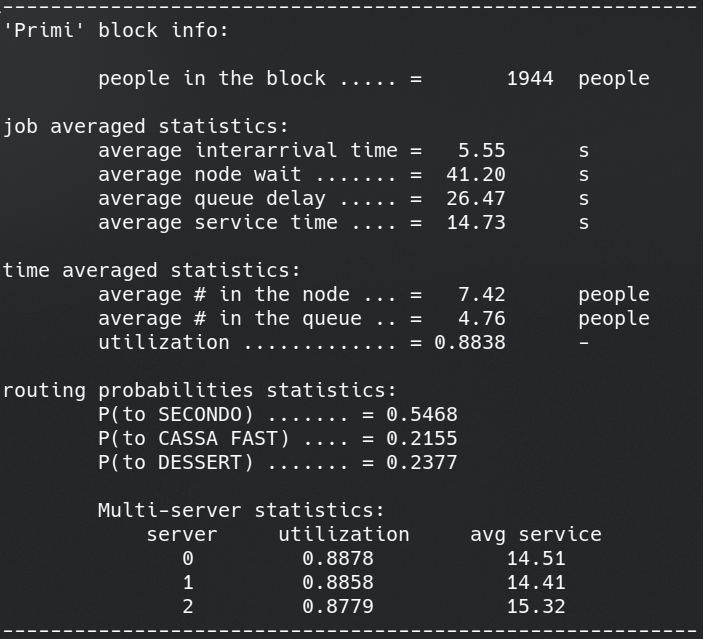
\includegraphics[width=.9\linewidth]{img/migliorativo_2_1/primo.png}
  \caption{Centro PRIMI.}
  \label{fig:primo_ext_2_pol_1}
\end{subfigure}
\begin{subfigure}{.5\textwidth}
  \centering
  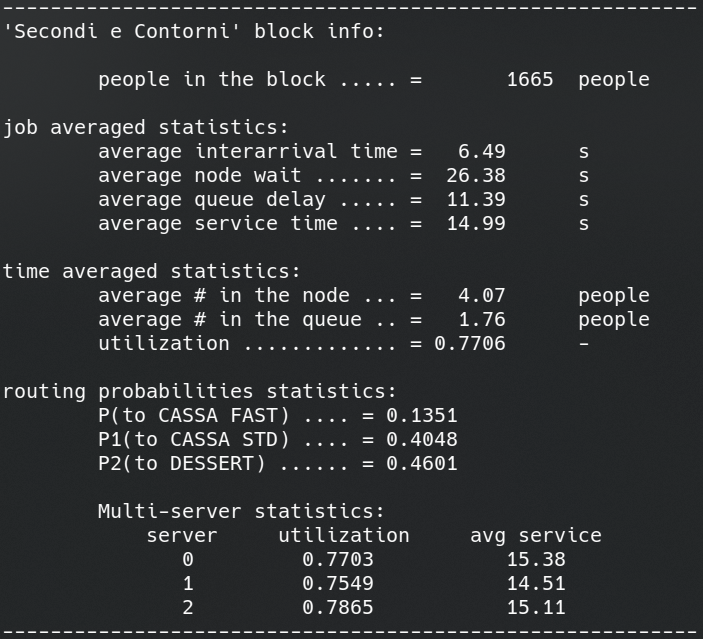
\includegraphics[width=.94\linewidth]{img/migliorativo_2_1/secondo.png}
  \caption{Centro SECONDI.}
  \label{fig:secondo_ext_2_pol_1}
\end{subfigure}
\begin{subfigure}{.5\textwidth}
  \centering
  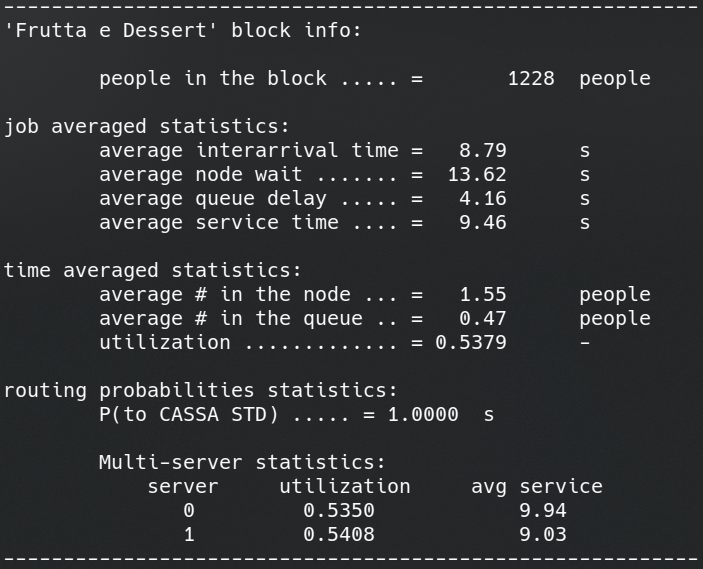
\includegraphics[width=.9\linewidth]{img/migliorativo_2_1/dessert.png}
  \caption{Centro DESSERT.}
  \label{fig:dessert_ext_2_plo_1}
\end{subfigure}
\begin{subfigure}{.5\textwidth}
  \centering
  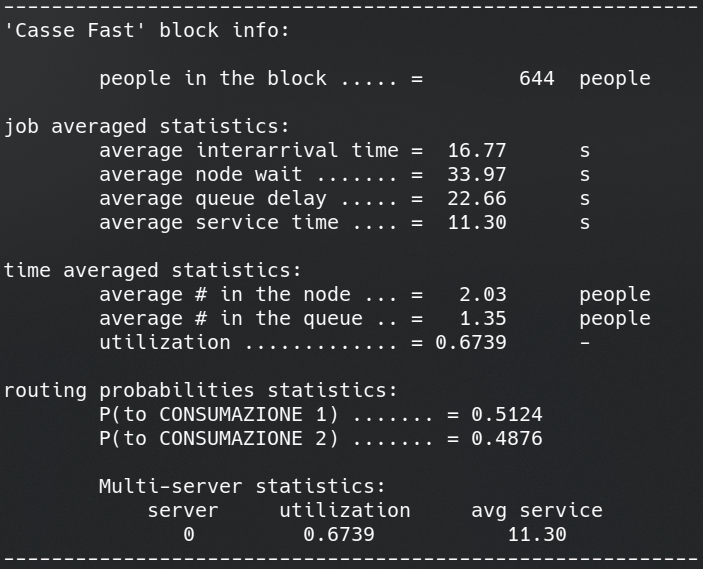
\includegraphics[width=.88\linewidth]{img/migliorativo_2_1/fast.png}
  \caption{Centro CASSA FAST.}
  \label{fig:cassa_fast_ext_2_pol_1}
\end{subfigure}
\begin{subfigure}{.5\textwidth}
  \centering
  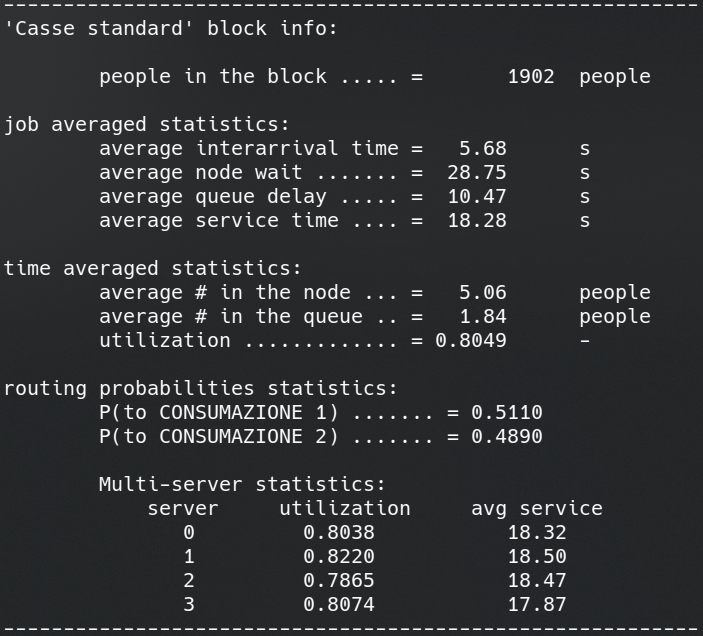
\includegraphics[width=.9\linewidth]{img/migliorativo_2_1/standard.png}
  \caption{Centro CASSA STD.}
  \label{fig:cassa_std_ext_2_pol_1}
\end{subfigure}
\caption{Statistiche di output per ogni centro.}
\label{fig:output_ext_2_pol_1}
\end{figure}

\begin{figure}[H]
\begin{subfigure}{.5\textwidth}
  \centering
  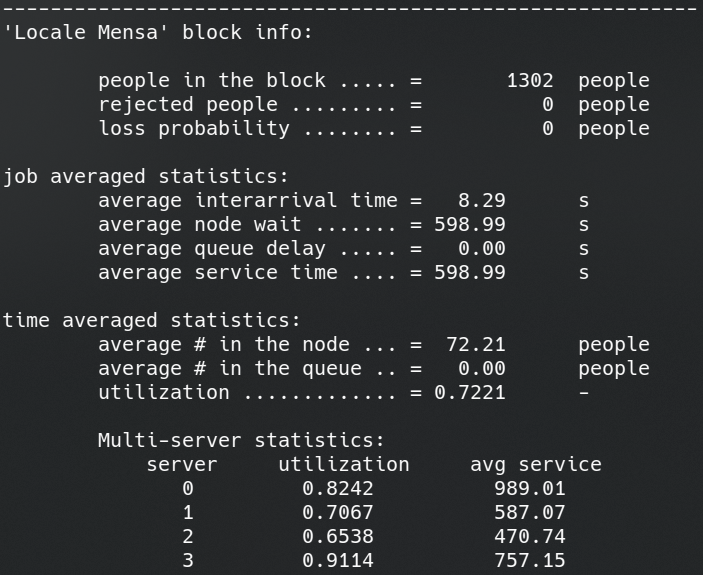
\includegraphics[width=.9\linewidth]{img/migliorativo_2_1/consumazione_1.png}
  \caption{centro CONSUMAZIONE 1 (solo i primi 4 posti).}
\end{subfigure}
\begin{subfigure}{.5\textwidth}
  \centering
  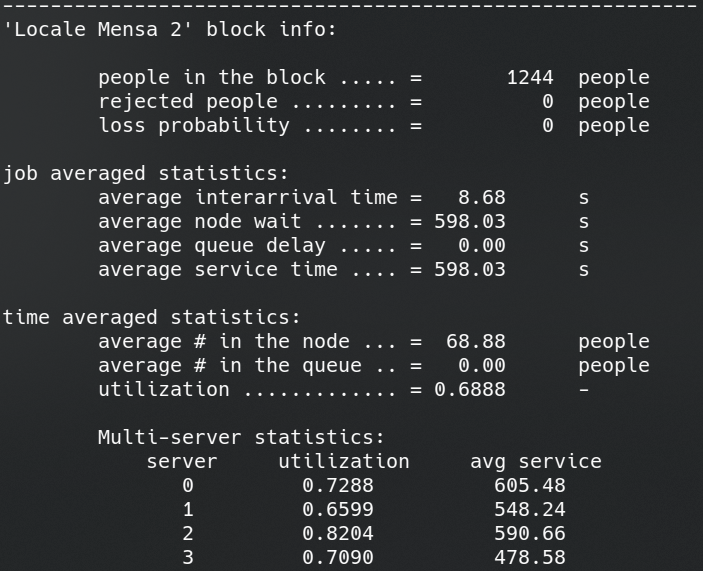
\includegraphics[width=.9\linewidth]{img/migliorativo_2_1/consumazione_2.png}
  \caption{centro CONSUMAZIONE 2 (solo i primi 4 posti).}
\end{subfigure}
\caption{Statistiche di output per ogni centro.}
\label{fig:output_ext_2_pol_1_consumazioni}
\end{figure}
\FloatBarrier
\subsubsection{Controlli di Consistenza}
I risultati per i \textbf{tempi di risposta} sono:
\begin{center}
\begin{tabular}{|c|c|c|c|}
 \hline
 \textbf{Centro} & \textbf{$E(T_{Q})$} & \textbf{$E(S)$} & \textbf{$E(T_{S})$}\\
 \hline
 \textit{PRIMO} & 26.47 & 14.73 & 41.20 \\
 \hline
 \textit{SECONDO} & 11.39 & 14.99 & 26.38\\
 \hline
 \textit{DESSERT} & 4.16 & 9.46 & 13.62\\
 \hline
 \textit{CASSA FAST} & 22.66 & 11.30 & 33.97\\
 \hline
 \textit{CASSA STD} & 10.47 & 18.28 & 28.75\\
 \hline
 \textit{CONSUMAZIONE 1} & 0 & 598.99 & 598.99\\
 \hline
 \textit{CONSUMAZIONE 2} & 0 & 598.03 & 598.03\\
 \hline
\end{tabular}
\end{center}
Mentre per le \textbf{popolazioni} dei centri:
\begin{center}
\begin{tabular}{|c|c|c|c|c|}
 \hline
 \textbf{Centro} & $E(N_{Q})$ & $m$ & $\rho$ & $E(N_{S})$\\
 \hline
 \textit{PRIMO} & 4.76 & \mP & 0.8838 & 7.41\\
 \hline
 \textit{SECONDO} & 1.76 & \mS & 0.7706 & 4.07\\
 \hline
 \textit{DESSERT} & 0.47 & \mD & 0.5379 & 1.55\\
 \hline
 \textit{CASSA FAST} & 1.35 & \mF & 0.6739 & 2.03\\
 \hline
 \textit{CASSA STD} & 1.84 & \mC & 0.8049 & 5.06\\
 \hline
 \textit{CONSUMAZIONE 1} & 0 & 100 & 0.7221 & 72.21\\
 \hline
 \textit{CONSUMAZIONE 2} & 0 & 100 & 0.6888 & 68.88\\
 \hline
\end{tabular}
\end{center}

\subsubsection{Dati di Input}
Il \textbf{numero di utenti}  nel sistema con due blocchi \textit{CONSUMAZIONE} e politica di scelta \textit{random} vale $2546$ ottenuto sommando il numero di arrivi nelle casse (vedi Fig. \ref{fig:cassa_fast_ext_2_pol_1} e Fig. \ref{fig:cassa_std_ext_2_pol_1}) oppure nei blocchi consumazione:

\[E(N_F) + E(N_C) = 644 + 1902 = 2546\]
\[E(N_{S_1}) + E(N_{S_2}) = 1302 + 1244 = 2546\]

Considerando i \textbf{tempi di servizio} dei soli tre serventi del centro \textit{PRIMO} (vedi Fig. \ref{fig:primo_ext_1}) si ottiene $E(S_{1}) = 14.51\ s$, $E(S_{2}) = 14.41\ s$, $E(S_{3}) = 15.32\ s$, dunque vicini al valore di riferimento $E(S) = 15\ s$. Inoltre, la media dei tempi restituisce il corrispettivo valore dell'intero blocco: $\frac{14.51 + 14.41 + 15.32}{3} = 14.73\ s$. Nella tabella che segue sono confrontati i \textbf{tassi di servizio} simulati e quelli passati come input.
\begin{center}
\begin{tabular}{|c|c|c|}
 \hline
 \textbf{Centro} & $\mu$ \textbf{Teorico} & $\mu$ \textbf{Simulato}\\
 \hline
 \textit{PRIMO} & \muP & 0.0678\\
 \hline
 \textit{SECONDO} & \muS & 0.0667\\
 \hline
 \textit{DESSERT} & \muD & 0.1057\\
 \hline
 \textit{CASSA FAST} & \muF & 0.0885\\
 \hline
 \textit{CASSA STD} & \muC & 0.0547\\
 \hline
 \textit{CONSUMAZIONE 1} & 0.001666 & 0.001669\\
 \hline
 \textit{CONSUMAZIONE 2} & 0.001666 & 0.001672\\
 \hline
\end{tabular}
\end{center}

Nella tabella che segue sono presentati i risultati per le \textbf{probabilità di routing}. Anche in questo caso i valori simulati sono in linea con i valori teorici.

\begin{center}
\begin{tabular}{|c|c|c|c|}
 \hline
 \textbf{Sorgente $i$} & \textbf{Destinazione $j$} & \textbf{\(p_{ij}\) Teorica} & \textbf{\(p_{ij}\) Simulata}\\
 \hline
 \textit{ESTERNO} & \textit{PRIMO}   & 0.7500 & 0.7635\\
 \hline
 \textit{ESTERNO} & \textit{SECONDO}   & 0.2500 & 0.2364\\
 \hline
 \textit{PRIMO} & \textit{SECONDO}   & 0.5500 & 0.5468\\
 \hline
 \textit{PRIMO} & \textit{DESSERT}   & 0.2500 & 0.2377\\
 \hline
 \textit{PRIMO} & \textit{CASSA FAST}   & 0.2000 & 0.2155\\
\hline
 \textit{SECONDO} & \textit{DESSERT}   & 0.4500 & 0.4601\\
 \hline
 \textit{SECONDO} & \textit{CASSA FAST}   & 0.1375 & 0.1351\\
\hline
 \textit{SECONDO} & \textit{CASSA STD}   & 0.4125 & 0.4048\\
\hline
 \textit{DESSERT} & \textit{CASSA STD}   & 1.0000 & 1.0000\\
 \hline
 \textit{CASSA FAST} & \textit{CONSUMAZIONE 1}   & 0.5000 & 0.5124\\
 \hline
 \textit{CASSA FAST} & \textit{CONSUMAZIONE 2}   & 0.5000 & 0.4876\\
 \hline
 \textit{CASSA STD} & \textit{CONSUMAZIONE 1}   & 0.5000 & 0.5110\\
 \hline
 \textit{CASSA STD} & \textit{CONSUMAZIONE 2}   & 0.5000 & 0.4890\\
 \hline
\end{tabular}
\end{center}
Per quanto riguarda i \textbf{tassi di arrivo} si ha che:
\begin{center}
\begin{tabular}{|c|c|c|}
 \hline
 \textbf{Centro} & $\lambda$ \textbf{Teorico} & $\lambda$ \textbf{Simulato}\\
 \hline
 \textit{PRIMO} & 0.1735 & 0.1799\\
 \hline
 \textit{SECONDO} & 0.1534 & 0.1541\\
 \hline
 \textit{DESSERT} & 0.1124 & 0.1136\\
 \hline
 \textit{CASSA FAST} & 0.0558 & 0.0595\\
 \hline
 \textit{CASSA STD} & 0.1757 & 0.1760\\
 \hline
 \textit{CONSUMAZIONE 1} & 0.1157 & 0.1204\\
 \hline
 \textit{CONSUMAZIONE 2} & 0.1157 & 0.1151\\
 \hline
\end{tabular}
\end{center}
I valori delle \textbf{visite medie} simulate e teoriche sono riportati di seguito:
\begin{center}
\begin{tabular}{|c|c|c|}
 \hline
 \textbf{Centro} & $v_i$ \textbf{Teorico} & $v_i$ \textbf{Simulato}\\
 \hline
 \textit{PRIMO} & 0.7500 & 0.7635\\
 \hline
 \textit{SECONDO} & 0.6625 & 0.6538\\
 \hline
 \textit{DESSERT} & 0.4856 & 0.4822\\
 \hline
 \textit{CASSA FAST} & 0.2410 & 0.2528\\
 \hline
 \textit{CASSA STD} & 0.7589 & 0.7468\\
 \hline
 \textit{CONSUMAZIONE 1} & 0.5000 & 0.5111\\
 \hline
 \textit{CONSUMAZIONE 2} & 0.5000 & 0.4884\\
 \hline
\end{tabular}
\end{center}


Nella tabella sottostante è possibile osservare come i valori simulati delle \textbf{utilizzazioni} si avvicinano ai valori teorici.
\begin{center}
\begin{tabular}{|c|c|c|}
 \hline
 \textbf{Centro} & $\rho$ \textbf{Teorica} & $\rho$ \textbf{Simulata}\\
 \hline
 \textit{PRIMO} & 0.8677 & 0.8838\\
 \hline
 \textit{SECONDO} & 0.7670 & 0.7706\\
 \hline
 \textit{DESSERT} & 0.5620 & 0.5379\\
 \hline
 \textit{CASSA FAST} & 0.6138 & 0.6739\\
 \hline
 \textit{CASSA STD} & 0.7906 & 0.8049\\
 \hline
 \textit{CONSUMAZIONE 1} & 0.6945 & 0.7211\\
 \hline
 \textit{CONSUMAZIONE 2} & 0.6945 & 0.6883\\
 \hline
\end{tabular}
\end{center}

\subsection{QoS}
Il \textbf{tempo di risposta globale} è pari a:
\[E(T_{r}^{(t)}) = \sum_{i=1}^{M} E(T_{i}) \cdot v_{i} \]
\[= E(T_1) \cdot v_1+ E(T_2) \cdot v_{2} + E(T_{3}) \cdot v_{3} + E(T_{F}) \cdot v_{F} + E(T_{C}) \cdot v_{C} + E(T_{S1}) \cdot v_{S1} + E(T_{S2}) \cdot v_{S2}\]
\[=  43.8488 \cdot 0.75 + 27.7345 \cdot 0.6625 + 14.6181 \cdot 0.4856 + 28.4897 \cdot 0.2410 + 30.4488 \cdot 0.7589 + 600 \cdot 0.5000 + 600 \cdot 0.5000\]
\[ = 688.2712\ s\]
Il risultato simulato è invece: 
\[E(T_{r}^{(s)}) = 683.8556\ s\]
Anche in questa configurazione la \textbf{probabilità di perdita} è:

\[p_{loss, S1}^{(t)} = p_{loss, S2}^{(t)} \simeq p_{loss, S1}^{(s)} = p_{loss, S2}^{(s)} = 0 \]

\section{Modello Migliorativo 2 con Politica Least Busy}

Rispetto a quanto discusso in Sec. \ref{sec:migliorativo_2_random}, la scelta dell'area dove consumare il pasto dipende dalle utilizzazioni. Infatti intuitivamente, un utente preferisce il locale meno occupato, in modo tale da aumentare le sue probabilità di trovare un posto a sedere.
Sia per il \textbf{modello concettuale} (vedi Fig. \ref{fig:esteso_2_concettuale}) che per il \textbf{modello delle specifiche} e il \textbf{modello computazionale} vale quanto già discusso in Sec. \ref{sec:migliorativo_2_random}.

\subsection{Verifica}

I dati ottenuti fanno riferimento ad una singola simulazione con durata pari al periodo di osservazione (i.e.,  3 ore) con seed pari a 123456789 (vedi Fig. \ref{fig:output_ext_2_pol_2} e Fig. \ref{fig:output_ext_2_pol_2_consumazioni}).

\begin{figure}[H]
\begin{subfigure}{.5\textwidth}
  \centering
  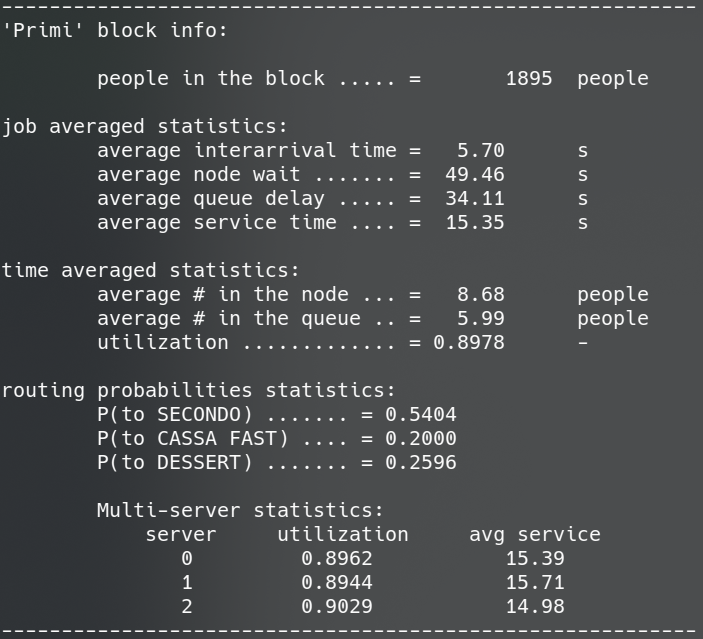
\includegraphics[width=.9\linewidth]{img/migliorativo_2_2/primo.png}
  \caption{Centro PRIMI.}
  \label{fig:primo_ext_2_pol_2}
\end{subfigure}
\begin{subfigure}{.5\textwidth}
  \centering
  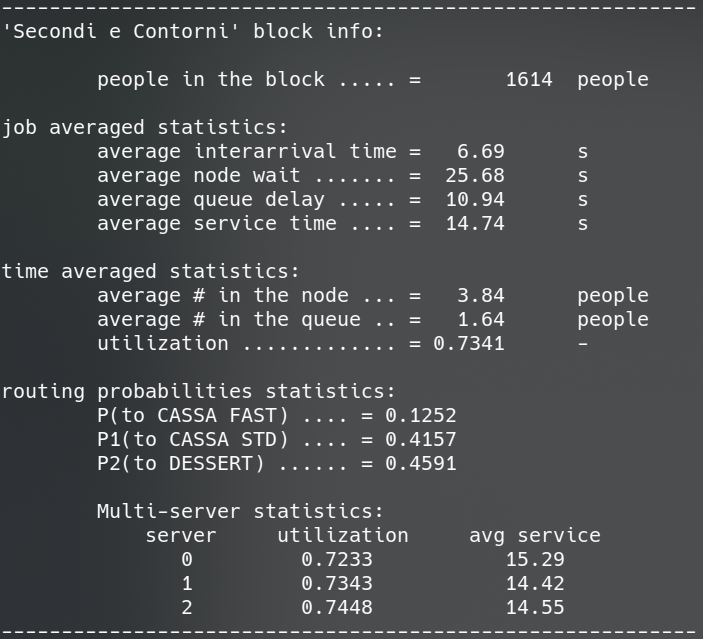
\includegraphics[width=.94\linewidth]{img/migliorativo_2_2/secondo.png}
  \caption{Centro SECONDI.}
  \label{fig:secondo_ext_2_pol_2}
\end{subfigure}
\begin{subfigure}{.5\textwidth}
  \centering
  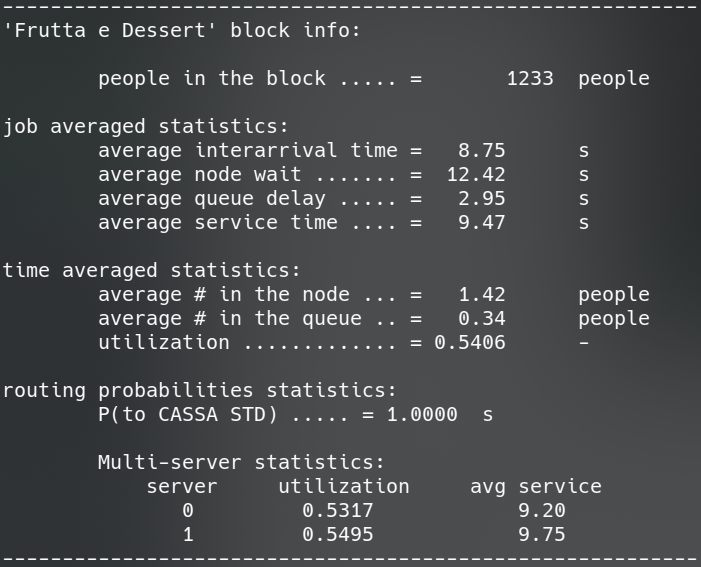
\includegraphics[width=.9\linewidth]{img/migliorativo_2_2/dessert.png}
  \caption{Centro DESSERT.}
  \label{fig:dessert_ext_2_plo_2}
\end{subfigure}
\begin{subfigure}{.5\textwidth}
  \centering
  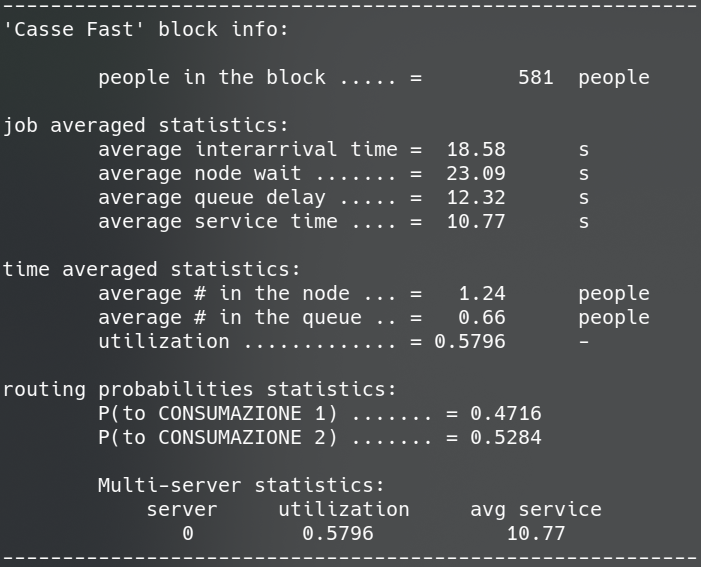
\includegraphics[width=.88\linewidth]{img/migliorativo_2_2/fast.png}
  \caption{Centro CASSA FAST.}
  \label{fig:cassa_fast_ext_2_pol_2}
\end{subfigure}
\begin{subfigure}{.5\textwidth}
  \centering
  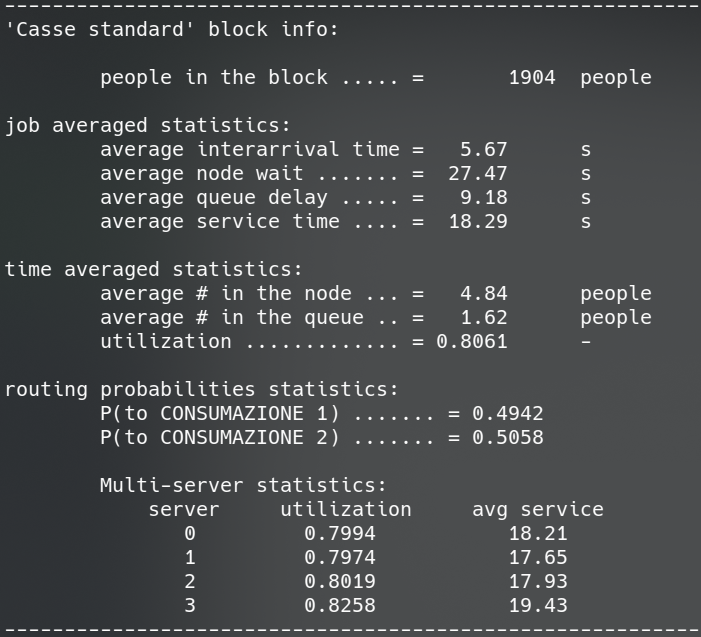
\includegraphics[width=.9\linewidth]{img/migliorativo_2_2/standard.png}
  \caption{Centro CASSA STD.}
  \label{fig:cassa_std_ext_2_pol_2}
\end{subfigure}
\caption{Statistiche di output per ogni centro.}
\label{fig:output_ext_2_pol_2}
\end{figure}

\begin{figure}[H]
\begin{subfigure}{.5\textwidth}
  \centering
  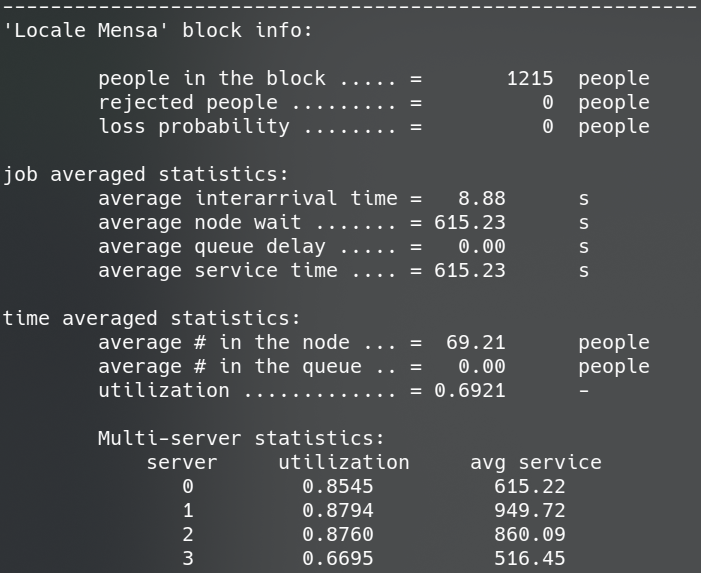
\includegraphics[width=.9\linewidth]{img/migliorativo_2_2/consumazione_1.png}
  \caption{centro CONSUMAZIONE 1 (solo i primi 4 posti).}
  \label{fig:consumazione_1_ext_2_pol_2}
\end{subfigure}
\begin{subfigure}{.5\textwidth}
  \centering
  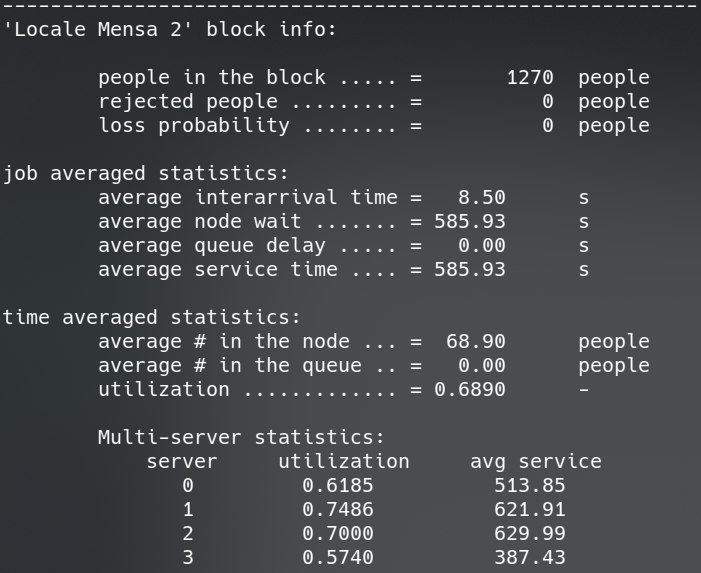
\includegraphics[width=.9\linewidth]{img/migliorativo_2_2/consumazione_2.png}
  \caption{centro CONSUMAZIONE 2 (solo i primi 4 posti).}
  \label{fig:consumazione_1_ext_2_pol_2}
\end{subfigure}
\caption{Statistiche di output per ogni centro.}
\label{fig:output_ext_2_pol_2_consumazioni}
\end{figure}
\FloatBarrier
\subsubsection{Controlli di Consistenza}
 
La condizione per i \textbf{tempi di risposta} è verificata per ogni blocco, come mostrato dai tempi simulati riportati di seguito:
\begin{center}
\begin{tabular}{|c|c|c|c|}
 \hline
 \textbf{Centro} & \textbf{$E(T_{Q})$} & \textbf{$E(S)$} & \textbf{$E(T_{S})$}\\
 \hline
 \textit{PRIMO} & 34.11 & 15.35 & 49.46 \\
 \hline
 \textit{SECONDO} & 10.94 & 14.74 & 25.68\\
 \hline
 \textit{DESSERT} & 2.95 & 9.47 & 12.42\\
 \hline
 \textit{CASSA FAST} & 12.32 & 10.77 & 23.09\\
 \hline
 \textit{CASSA STD} & 9.18 & 18.29 & 27.47\\
 \hline
 \textit{CONSUMAZIONE 1} & 0 & 615.23 & 615.23\\
 \hline
 \textit{CONSUMAZIONE 2} & 0 & 585.93 & 585.93\\
 \hline
\end{tabular}
\end{center}
Come anche per le \textbf{popolazioni} dei centri:
\begin{center}
\begin{tabular}{|c|c|c|c|c|}
 \hline
 \textbf{Centro} & $E(N_{Q})$ & $m$ & $\rho$ & $E(N_{S})$\\
 \hline
 \textit{PRIMO} & 5.99 & \mP & 0.8978 & 8.68\\
 \hline
 \textit{SECONDO} & 1.64 & \mS & 0.7341 & 3.84\\
 \hline
 \textit{DESSERT} & 0.34 & \mD & 0.5406 & 1.42\\
 \hline
 \textit{CASSA FAST} & 0.66 & \mF & 0.5796 & 1.24\\
 \hline
 \textit{CASSA STD} & 1.62 & \mC & 0.8061 & 4.84\\
 \hline
 \textit{CONSUMAZIONE 1} & 0 & 100 & 0.6921 & 69.21\\
 \hline
 \textit{CONSUMAZIONE 2} & 0 & 100 & 0.6890 & 68.90\\
 \hline
\end{tabular}
\end{center}

\subsubsection{Dati di Input}

Il \textbf{numero di utenti} entrato nel sistema è $2485$ ottenuto sommando il numero di arrivi per i centri \textit{CASSA FAST} e \textit{CASSA STD} (vedi Fig. \ref{fig:cassa_fast_ext_2_pol_2} e Fig. \ref{fig:cassa_std_ext_2_pol_2}): $581 + 1904 = 2485$. 

Con i \textbf{tempi di servizio} del centro \textit{PRIMO} (vedi Fig. \ref{fig:primo_ext_2_pol_2}) si ottiene $E(S_{1}) = 15.39\ s$, $E(S_{2}) = 15.71\ s$, $E(S_{3}) = 14.98\ s$, dunque vicini al valore di riferimento $E(S) = 15\ s$. Inoltre, la media dei tempi restituisce il corrispettivo valore dell'intero blocco: $\frac{15.39 + 15.71 + 14.98}{3} = 15.35\ s$. 
Di seguito sono confrontati i \textbf{tassi di servizio} simulati e quelli passati in input.
\begin{center}
\begin{tabular}{|c|c|c|}
 \hline
 \textbf{Centro} & $\mu$ \textbf{Teorico} & $\mu$ \textbf{Simulato}\\
 \hline
 \textit{PRIMO} & \muP & 0.0651\\
 \hline
 \textit{SECONDO} & \muS & 0.0678\\
 \hline
 \textit{DESSERT} & \muD & 0.1056\\
 \hline
 \textit{CASSA FAST} & \muF & 0.0928\\
 \hline
 \textit{CASSA STD} & \muC & 0.05467\\
 \hline
 \textit{CONSUMAZIONE 1} & 0.001666 & 0.001625\\
 \hline
 \textit{CONSUMAZIONE 2} & 0.001666 & 0.001706\\
 \hline
\end{tabular}
\end{center}

Nella tabella che segue sono presentati i risultati per le \textbf{probabilità di routing}. Anche in questo caso i valori simulati sono in linea con i valori teorici.
\begin{center}
\begin{tabular}{|c|c|c|c|}
 \hline
 \textbf{Sorgente $i$} & \textbf{Destinazione $j$} & \textbf{\(p_{ij}\) Teorica} & \textbf{\(p_{ij}\) Simulata}\\
 \hline
 \textit{ESTERNO} & \textit{PRIMO}   & 0.7500 & 0.7625\\
 \hline
 \textit{ESTERNO} & \textit{SECONDO}   & 0.2500 & 0.2374\\
 \hline
 \textit{PRIMO} & \textit{SECONDO}   & 0.5500 & 0.5404\\
 \hline
 \textit{PRIMO} & \textit{DESSERT}   & 0.2500 & 0.2596\\
 \hline
 \textit{PRIMO} & \textit{CASSA FAST}   & 0.2000 & 0.2000\\
\hline
 \textit{SECONDO} & \textit{DESSERT}   & 0.4500 & 0.4591\\
 \hline
 \textit{SECONDO} & \textit{CASSA FAST}   & 0.1375 & 0.1252\\
\hline
 \textit{SECONDO} & \textit{CASSA STD}   & 0.4125 & 0.4157\\
\hline
 \textit{DESSERT} & \textit{CASSA STD}   & 1.0000 & 1.0000\\
 \hline
 \textit{CASSA FAST} & \textit{CONSUMAZIONE 1}   & 0.5000 & 0.4716\\
 \hline
 \textit{CASSA FAST} & \textit{CONSUMAZIONE 2}   & 0.5000 & 0.5284\\
 \hline
 \textit{CASSA STD} & \textit{CONSUMAZIONE 1}   & 0.5000 & 0.4942\\
 \hline
 \textit{CASSA STD} & \textit{CONSUMAZIONE 2}   & 0.5000 & 0.5058\\
 \hline
\end{tabular}
\end{center}
Per quanto riguarda i \textbf{tassi di arrivo} si ha che:
\begin{center}
\begin{tabular}{|c|c|c|}
 \hline
 \textbf{Centro} & $\lambda$ \textbf{Teorico} & $\lambda$ \textbf{Simulato}\\
 \hline
 \textit{PRIMO} & 0.1735 & 0.1754\\
 \hline
 \textit{SECONDO} & 0.1534 & 0.1493\\
 \hline
 \textit{DESSERT} & 0.1124 & 0.1140\\
 \hline
 \textit{CASSA FAST} & 0.0558 & 0.0537\\
 \hline
 \textit{CASSA STD} & 0.1757 & 0.1761\\
 \hline
 \textit{CONSUMAZIONE 1} & 0.1157 & 0.1124\\
 \hline
 \textit{CONSUMAZIONE 2} & 0.1157 & 0.1175\\
 \hline
\end{tabular}
\end{center}
E' possibile osservare i valori delle \textbf{visite medie} simulate e teoriche:
\begin{center}
\begin{tabular}{|c|c|c|}
 \hline
 \textbf{Centro} & $v_i$ \textbf{Teorico} & $v_i$ \textbf{Simulato}\\
 \hline
 \textit{PRIMO} & 0.7500 & 0.7625\\
 \hline
 \textit{SECONDO} & 0.6625 & 0.6494\\
 \hline
 \textit{DESSERT} & 0.4856 & 0.4960\\
 \hline
 \textit{CASSA FAST} & 0.2410 & 0.2338\\
 \hline
 \textit{CASSA STD} & 0.7589 & 0.7659\\
 \hline
 \textit{CONSUMAZIONE 1} & 0.5000 & 0.4887\\
 \hline
 \textit{CONSUMAZIONE 2} & 0.5000 & 0.5109\\
 \hline
\end{tabular}
\end{center}

Nella tabella sottostante è possibile osservare come i valori simulati delle \textbf{utilizzazioni} si avvicinano ai valori teorici.
\begin{center}
\begin{tabular}{|c|c|c|}
 \hline
 \textbf{Centro} & $\rho$ \textbf{Teorica} & $\rho$ \textbf{Simulata}\\
 \hline
 \textit{PRIMO} & 0.8677 & 0.8978\\
 \hline
 \textit{SECONDO} & 0.7670 & 0.7341\\
 \hline
 \textit{DESSERT} & 0.5620 & 0.5406\\
 \hline
 \textit{CASSA FAST} & 0.6138 & 0.5796\\
 \hline
 \textit{CASSA STD} & 0.7906 & 0.8061\\
 \hline
 \textit{CONSUMAZIONE 1} & 0.6945 & 0.6921\\
 \hline
 \textit{CONSUMAZIONE 2} & 0.6945 & 0.6890\\
 \hline
\end{tabular}
\end{center}
\subsection{QoS}
Per il \textbf{tempo di risposta globale} si ha: 
\[E(T_{r}^{(t)}) = \sum_{i=1}^{M} E(T_{i}) \cdot v_{i} \]
\[= E(T_1) \cdot v_1+ E(T_2) \cdot v_{2} + E(T_{3}) \cdot v_{3} + E(T_{F}) \cdot v_{F} + E(T_{C}) \cdot v_{C} + E(T_{S1}) \cdot v_{S1} + E(T_{S2}) \cdot v_{S2}\]
\[=  43.8488 \cdot 0.75 + 27.7345 \cdot 0.6625 + 14.6181 \cdot 0.4856 + 28.4897 \cdot 0.2410 + 30.4488 \cdot 0.7589 + 600 \cdot 0.5000 + 600 \cdot 0.5000\]
\[ = 688.2712\ s\]
Il risultato simulato è invece: 
\[E(T_{r}^{(s)}) = 687.2456\ s\]
Anche in questa configurazione la \textbf{probabilità di perdita} è:
\[p_{loss, S1}^{(t)} = p_{loss, S2}^{(t)} \simeq p_{loss, S1}^{(s)} = p_{loss, S2}^{(s)} = 0 \]

\section{Risultati}

Sono ora analizzati i risultati ottenuti nei modelli migliorativi, anche confrontandoli con il modello base da cui si è partiti.

\subsection{Simulazione finite-horizon}

Nelle Fig. \ref{fig:grt_finite_200_replicas}, \ref{fig:ext_grt_finite_m21_replicas} e \ref{fig:ext_grt_finite_m22_replicas} sono mostrati i valori degli intervalli di confidenza all'aumentare del numero di \textbf{repliche}. 
Per i tempi di risposta vale quanto già detto riguardo al modello base e in particolare questi si discostano dal tempo di risposta stazionario teorico in quanto il tempo di simulazione di tre ore è troppo breve e quindi è ancora presente un bias rispetto allo stato iniziale della rete.  

Per un ensemble con 10000 repliche, il tempo di risposta \textbf{transiente} è \(686.869893 \pm 0.314576\).
\begin{figure}[H]
  \centering
  \includesvg[inkscapelatex=false, width = 370pt]{grt_finite_200_replicas.svg}
  \caption{Intervalli di confidenza del tempo globale di risposta della rete all'aumentare del numero di repliche per il modello migliorativo con 200 posti nel blocco \textit{CONSUMAZIONE}.}
  \label{fig:grt_finite_200_replicas}
\end{figure}

\begin{figure}[H]
  \centering
  \includesvg[inkscapelatex=false, width = 370pt]{ext_grt_finite_m21_replicas.svg}
  \caption{Intervalli di confidenza del tempo globale di risposta della rete all'aumentare del numero di repliche per il modello migliorativo 2 con politica random.}
  \label{fig:ext_grt_finite_m21_replicas}
\end{figure}

\begin{figure}[H]
  \centering
  \includesvg[inkscapelatex=false, width = 370pt]{ext_grt_finite_m22_replicas.svg}
  \caption{Intervalli di confidenza del tempo globale di risposta della rete all'aumentare del numero di repliche per il modello migliorativo 2 con politica least busy.}
  \label{fig:ext_grt_finite_m22_replicas}
\end{figure}

Nelle Fig. \ref{fig:ext_grt_seed_finite_200}, \ref{fig:ext_grt_seed_finite_m21} e \ref{fig:ext_grt_seed_finite_m22} vengono presentati gli andamenti dei valori per i \textbf{seed} al passare del tempo. 
Per il modello migliorativo 1 i tempi per una singola simulazione hanno un andamento che tende al valore teorico, a differenza degli altri.

\begin{figure}[H]
  \centering
  \includesvg[inkscapelatex=false, width = 370pt]{ext_grt_seed_finite_200.svg}
  \caption{Andamento del tempo globale di risposta al variare del seed di sistema per il modello migliorativo con 200 posti a sedere.}
  \label{fig:ext_grt_seed_finite_200}
\end{figure}

\begin{figure}[H]
  \centering
  \includesvg[inkscapelatex=false, width = 370pt]{ext_grt_seed_finite_m21.svg}
  \caption{Andamento del tempo globale di risposta al variare del seed di sistema per il modello migliorativo 2 con politica random.}
  \label{fig:ext_grt_seed_finite_m21}
\end{figure}

\begin{figure}[H]
  \centering
  \includesvg[inkscapelatex=false, width = 370pt]{ext_grt_seed_finite_m22.svg}
  \caption{Andamento del tempo globale di risposta al variare del seed di sistema per il modello migliorativo 2 con politica least busy.}
  \label{fig:ext_grt_seed_finite_m22}
\end{figure}
\subsection{Simulazione Infinite-Horizon}
Infine sono confrontati i tempi dei quattro modello studiati (vedi Fig. \ref{fig:ext_grt_infinite_batch}) nella \textbf{simulazione infinita}.
Il grafico mostra una convergenza per i modelli migliorativi al valore teorico, con quest'ultimo più elevato rispetto al modello iniziale. 
Questo incremento è dovuto al maggior numero di dipendenti che consuma il pasto e dunque a tempi di servizio aggiuntivi rispetto al modello base. 

\begin{figure}[H]
  \centering
  \includesvg[inkscapelatex=false, width = 370pt]{ext_grt_infinite_batch.svg}
  \caption{Andamento del tempo globale di risposta medio all'aumentare del numero di batch per i quattro modelli.}
  \label{fig:ext_grt_infinite_batch}
\end{figure}

Gli intervalli di confidenza al variare del seed nella simulazione infinite sono riportati in Fig. \ref{fig:grt_seed_infinite_200}, \ref{fig:ext_grt_seed_infinite_m21} e \ref{fig:ext_grt_seed_infinite_m22}.

\begin{figure}[H]
  \centering
  \includesvg[inkscapelatex=false, width = 370pt]{grt_seed_infinite_200.svg}
  \caption{Intervalli di confidenza per il tempo globale di risposta medio al variare del seed per il modello migliorativo 1.}
  \label{fig:grt_seed_infinite_200}
\end{figure}

\begin{figure}[H]
  \centering
  \includesvg[inkscapelatex=false, width = 370pt]{ext_grt_seed_infinite_m21.svg}
  \caption{Intervalli di confidenza per il tempo globale di risposta medio al variare del seed per il modello migliorativo 2 con politica random.}
  \label{fig:ext_grt_seed_infinite_m21}
\end{figure}

\begin{figure}[H]
  \centering
  \includesvg[inkscapelatex=false, width = 370pt]{ext_grt_seed_infinite_m22.svg}
  \caption{Intervalli di confidenza per il tempo globale di risposta medio al variare del seed per il modello migliorativo 2 con politica least busy.}
  \label{fig:ext_grt_seed_infinite_m22}
\end{figure}

\subsection{Probabilità di Perdita}

Dall'analisi dei risultati conseguiti nei modelli migliorativi, si è visto come la probabilità di perdita sia nulla. Tutti i dipendenti dunque trovano un posto a sedere dove poter consumare il proprio pasto.  
Non sono cosi riportati grafici di alcun genere.

\section{Conclusioni}

Riassumendo il lavoro svolto, si è partiti da un modello base dal quale si sono estrapolati i dati necessari per analizzarlo, trovando cosi delle limitazioni. In seguito, sono stati definiti tre modelli migliorativi, ognuno con una sua implementazione specifica, che annullano la probabilità di perdita a scapito di un aumento del tempo di risposta globale.

Un'ultima osservazione riguarda la progettazione del sistema, in particolare la mancata considerazione dei \textbf{costi} di mantenimento e manutenzione, che sicuramente incidono sulle scelte da fare. 

\end{document}